%----------
%   IMPORTANTE
%----------

% Esta plantilla está basada en las recomendaciones de la guía "Trabajo fin de Grado: Escribir el TFG", que encontrarás en http://uc3m.libguides.com/TFG/escribir
% contiene recomendaciones de la Biblioteca basadas principalmente en estilos APA e IEEE, pero debes seguir siempre las orientaciones de tu Tutor de TFG y la normativa de TFG para tu titulación.



% ESTA PLANTILLA ESTÁ BASADA EN EL ESTILO IEEE


%----------
%	CONFIGURACIÓN DEL DOCUMENTO
%----------

\documentclass[12pt]{report} % fuente a 12pt

\usepackage{xurl}


% MÁRGENES: 2,5 cm sup. e inf.; 3 cm izdo. y dcho.
\usepackage[
a4paper,
vmargin=2.5cm,
hmargin=3cm
]{geometry}

% INTERLINEADO: Estrecho (6 ptos./interlineado 1,15) o Moderado (6 ptos./interlineado 1,5)
\renewcommand{\baselinestretch}{1.15}
\parskip=6pt

% DEFINICIÓN DE COLORES para portada y listados de código
\usepackage[table]{xcolor}
\definecolor{azulUC3M}{RGB}{0,0,102}
\definecolor{gray97}{gray}{.97}
\definecolor{gray75}{gray}{.75}
\definecolor{gray45}{gray}{.45}

% Soporte para GENERAR PDF/A --es importante de cara a su inclusión en e-Archivo porque es el formato óptimo de preservación y a la generación de metadatos, tal y como se describe en http://uc3m.libguides.com/ld.php?content_id=31389625. 

% En la plantilla incluimos el archivo OUTPUT.XMPDATA. Puedes descargar este archivo e incluir los metadatos que se incorporarán al archivo PDF cuando compiles el archivo memoria.tex. Después vuelve a subirlo a tu proyecto. 
\usepackage[a-1b]{pdfx}

% ENLACES
\usepackage{hyperref}
\hypersetup{colorlinks=true,
	linkcolor=black, % enlaces a partes del documento (p.e. índice) en color negro
	urlcolor=blue} % enlaces a recursos fuera del documento en azul

% EXPRESIONES MATEMÁTICAS
\usepackage{amsmath,amssymb,amsfonts,amsthm}

% Codificación caracteres
\usepackage{txfonts} 
\usepackage[T1]{fontenc}
\usepackage[utf8]{inputenc}


%gaus diagrama

\usepackage{pgfplots}
\pgfplotsset{compat=1.18}


% diagrama gant
\usepackage{pgfgantt}
\usepackage{pdflscape}
\usepackage{afterpage}

\usepackage{fancyhdr}
\usepackage{graphicx}


\usepackage{tabularx}
\usepackage{enumitem}


\fancypagestyle{landscape}{
  \fancyhf{}
  \renewcommand{\headrulewidth}{0pt}
  \fancyhead[R]{%
    \rotatebox{90}{\thepage}
  }
}

% Definición idioma español
\usepackage[spanish, es-tabla]{babel} 
\usepackage[babel, spanish=spanish]{csquotes}
\AtBeginEnvironment{quote}{\small}

% diseño de PIE DE PÁGINA
\usepackage{fancyhdr}
\pagestyle{fancy}
\fancyhf{}
\renewcommand{\headrulewidth}{0pt}
\rfoot{\thepage}
\fancypagestyle{plain}{\pagestyle{fancy}}

% DISEÑO DE LOS TÍTULOS de las partes del trabajo (capítulos y epígrafes o subcapítulos)
\usepackage{titlesec}
\usepackage{titletoc}
\titleformat{\chapter}[block]
{\large\bfseries\filcenter}
{\thechapter.}
{5pt}
{\MakeUppercase}
{}
\titlespacing{\chapter}{0pt}{0pt}{*3}
\titlecontents{chapter}
[0pt]                                               
{}
{\contentsmargin{0pt}\thecontentslabel.\enspace\uppercase}
{\contentsmargin{0pt}\uppercase}                        
{\titlerule*[.7pc]{.}\contentspage}                 

\titleformat{\section}
{\bfseries}
{\thesection.}
{5pt}
{}
\titlecontents{section}
[5pt]                                               
{}
{\contentsmargin{0pt}\thecontentslabel.\enspace}
{\contentsmargin{0pt}}
{\titlerule*[.7pc]{.}\contentspage}

\titleformat{\subsection}
{\normalsize\bfseries}
{\thesubsection.}
{5pt}
{}
\titlecontents{subsection}
[10pt]                                               
{}
{\contentsmargin{0pt}                          
	\thecontentslabel.\enspace}
{\contentsmargin{0pt}}                        
{\titlerule*[.7pc]{.}\contentspage}  


% DISEÑO DE TABLAS
\usepackage{multirow} % permite combinar celdas 
\usepackage{caption} % para personalizar el título de tablas y figuras
\usepackage{floatrow} % utilizamos este paquete y sus macros \ttabbox y \ffigbox para alinear los nombres de tablas y figuras de acuerdo con el estilo definido.
\usepackage{array} % con este paquete podemos definir en la siguiente línea un nuevo tipo de columna para tablas: ancho personalizado y contenido centrado
\newcolumntype{P}[1]{>{\centering\arraybackslash}p{#1}}
\newcolumntype{Q}[1]{>{\centering\arraybackslash}p{\dimexpr#1\linewidth-2\tabcolsep\relax}}
\DeclareCaptionFormat{upper}{#1#2\uppercase{#3}\par}

% Diseño de tabla para ingeniería
\captionsetup*[table]{
	format=upper,
	name=TABLA,
	justification=centering,
	labelsep=period,
	width=.75\linewidth,
	labelfont=small,
	font=small
}
\usepackage{booktabs}
\usepackage[flushleft]{threeparttable}

% DISEÑO DE FIGURAS. 
\usepackage{graphicx}
\graphicspath{{imagenes/}} % ruta a la carpeta de imágenes

% Diseño de figuras para ingeniería
\captionsetup[figure]{
	format=hang,
	name=Fig.,
	singlelinecheck=off,
	labelsep=period,
	labelfont=small,
	font=small		
}

\usepackage{svg}

% NOTAS A PIE DE PÁGINA
\usepackage{chngcntr} % para numeración continua de las notas al pie
\counterwithout{footnote}{chapter}

% LISTADOS DE CÓDIGO
% soporte y estilo para listados de código. Más información en https://es.wikibooks.org/wiki/Manual_de_LaTeX/Listados_de_código/Listados_con_listings
\usepackage{listings}

% definimos un estilo de listings
\lstdefinestyle{estilo}{ frame=Ltb,
	framerule=0pt,
	aboveskip=0.5cm,
	framextopmargin=3pt,
	framexbottommargin=3pt,
	framexleftmargin=0.4cm,
	framesep=0pt,
	rulesep=.4pt,
	backgroundcolor=\color{gray97},
	rulesepcolor=\color{black},
	%
	basicstyle=\ttfamily\footnotesize,
	keywordstyle=\bfseries,
	stringstyle=\ttfamily,
	showstringspaces = false,
	commentstyle=\color{gray45},     
	%
	numbers=left,
	numbersep=15pt,
	numberstyle=\tiny,
	numberfirstline = false,
	breaklines=true,
	xleftmargin=\parindent
}

\usepackage{tikz}
\usetikzlibrary{shapes,arrows,positioning}

\usepackage{dirtree}

\captionsetup*[lstlisting]{font=small, labelsep=period}
% fijamos el estilo a utilizar 
\lstset{style=estilo}
\renewcommand{\lstlistingname}{\uppercase{Código}}

\usepackage{longtable}

%BIBLIOGRAFÍA 

% CONFIGURACIÓN PARA LA BIBLIOGRAFÍA IEEE
\usepackage[backend=biber, style=ieee, isbn=false,sortcites, maxbibnames=6, minbibnames=1,
maxcitenames=2,mincitenames=1]{biblatex} % Configuración para el estilo de citas de IEEE, recomendado para el área de ingeniería. "maxbibnames" indica que a partir de 6 autores trunque la lista en el primero (minbibnames) y añada "et al." tal y como se utiliza en el estilo IEEE.

% Añadimos las siguientes indicaciones para mejorar la adaptación del estilos en español
\DefineBibliographyStrings{spanish}{%
	andothers = {et\addabbrvspace al\adddot}
}
\DefineBibliographyStrings{spanish}{
	url = {\adddot\space[En línea]\adddot\space Disponible en:}
}
\DefineBibliographyStrings{spanish}{
	urlseen = {Acceso:}
}
\DefineBibliographyStrings{spanish}{
	pages = {pp\adddot},
	page = {p.\adddot}
}

\addbibresource{referencias.bib} % llama al archivo referencias.bib en el que deberá estar la bibliografía utilizada


%-------------
%	DOCUMENTO
%-------------

\begin{document}
\pagenumbering{roman} % Se utilizan cifras romanas en la numeración de las páginas previas al cuerpo del trabajo
	
%----------
%	PORTADA
%----------	
\begin{titlepage}
	\begin{sffamily}
	\color{azulUC3M}
	\begin{center}
		\begin{figure}[H] %incluimos el logotipo de la Universidad
			\makebox[\textwidth][c]{
\includegraphics[width=16cm]{logo_UC3M.png}}
		\end{figure}
		\vspace{2.5cm}
		\begin{Large}
			Grado Universitario en Ingeniería Informática\\			
			 2025-2026\\ %Indica el curso académico
			\vspace{2cm}		
			\textsl{Trabajo Fin de Grado}
			\bigskip
			
		\end{Large}
		 	{\Huge ``Sistema Multi-Agente de simulación de autobuses para evaluación de la dotación programada mediante KPIs''}\\
		 	\vspace*{0.5cm}
	 		\rule{10.5cm}{0.1mm}\\
			\vspace*{0.9cm}
			{\LARGE Héctor Álvarez Marcos}\\ 
			\vspace*{1cm}
		\begin{Large}
			Tutor\\
			Javier Ignacio Carbó Rubiera\\
			Colmenarejo, Septiembre 2026\\
		\end{Large}
	\end{center}
	\vfill
	\color{black}
	% SI NUESTRO TRABAJO SE VA A PUBLICAR CON UNA LICENCIA CREATIVE COMMONS, INCLUIR ESTAS LÍNEAS. ES LA OPCIÓN RECOMENDADA.
	
\includegraphics[width=4.2cm]{creativecommons.png}\\ %incluimos el logotipo de Creative Commons
	Esta obra se encuentra sujeta a la licencia Creative Commons \textbf{Reconocimiento - No Comercial - Sin Obra Derivada}
	\end{sffamily}
\end{titlepage}

\newpage %página en blanco o de cortesía
\thispagestyle{empty}
\mbox{}

%----------
%	RESUMEN Y PALABRAS CLAVE
%----------	
\renewcommand\abstractname{\large\bfseries\filcenter\uppercase{Resumen}}
\begin{abstract}
\thispagestyle{plain}
\setcounter{page}{3}
	
El presente trabajo determina en qué medida un sistema multiagente parametrizado
con datos operacionales reales es capaz de reproducir el comportamiento observado
de una línea de autobús urbano y de sostener el cálculo de indicadores clave de
rendimiento sobre la dotación programada, cuya adecuación a la demanda resulta
difícil de contrastar mediante el análisis descriptivo de los registros históricos.

Partiendo de ocho meses de datos operacionales de la línea E01 de la Empresa
Municipal de Transportes de Madrid, se caracteriza la demanda de cada parada y
franja horaria mediante el ajuste de distribuciones normal, binomial negativa y
geométrica, seleccionadas por criterio de información de Akaike tras el contraste
de hipótesis correspondiente. Sobre esa parametrización se diseñan e implementan
dos arquitecturas multiagente en la plataforma GAMA, comunicadas mediante
protocolos FIPA. La primera presenta representación individual del pasajero y la
segunda utiliza demanda agregada en la parada. Ambas se ejecutan
bajo un esquema de simulación de Monte Carlo de mil réplicas, del que se derivan
los indicadores de ocupación, regularidad, tiempo de espera y pasajeros residuales,
explotados a través de una herramienta web de visualización.

La fidelidad del modelo se evalúa comparando las distribuciones de ocupación
simuladas y observadas mediante el coeficiente de Bhattacharyya. Los resultados
reproducen el nivel medio observado con un déficit medio de 2,01 pasajeros,
equivalente a 0,13 desviaciones típicas, y una sobredispersión creciente atribuible
al muestreo independiente de subidas y bajadas, que omite la covarianza negativa
presente en la operación real. Ambas arquitecturas producen resultados equivalentes,
siendo la agregada 4,3 veces más rápida.

Se concluye que el modelo sostiene el análisis del nivel medio de ocupación y la
comparación relativa entre configuraciones, pero no la estimación de percentiles
extremos ni el análisis de escenarios que alteren la oferta.
    
	\textbf{Palabras clave:}
	Sistemas multi-agente, simulación de Monte Carlo, transporte público urbano, transporte inteligente,
	indicadores clave de rendimiento, GAMA
    
    

	\vfill
\end{abstract}
	\newpage % página en blanco o de cortesía
	\thispagestyle{empty}
	\mbox{}


%----------
%	DEDICATORIA
%----------	
\chapter*{Agradecimientos} % \chapter* evita que aparezca en el índice

\setcounter{page}{5}
	
	% ESCRIBIR LA DEDICATORIA AQUÍ	
		
	\vfill
	
	\newpage % página en blanco o de cortesía
	\thispagestyle{empty}
	\mbox{}
	

%----------
%	ÍNDICES
%----------	

%--
% Índice general
%-
\tableofcontents
\thispagestyle{fancy}

\newpage % página en blanco o de cortesía
\thispagestyle{empty}
\mbox{}

%--
% Índice de figuras. Si no se incluyen, comenta las líneas siguientes
%-
\listoffigures
\thispagestyle{fancy}

\newpage % página en blanco o de cortesía
\thispagestyle{empty}
\mbox{}

%--
% Índice de tablas. Si no se incluyen, comenta las líneas siguientes
%-
\listoftables
\thispagestyle{fancy}

\newpage % página en blanco o de cortesía
\thispagestyle{empty}
\mbox{}


\chapter*{Lista de acrónimos}
\thispagestyle{fancy}

\begin{longtable}{@{}p{2.5cm}p{\dimexpr\textwidth-3cm\relax}@{}}
\textbf{ABM}   & \textit{Agent-Based Model}. Modelo basado en agentes \\
\textbf{ACL}   & \textit{Agent Communication Language}. Lenguaje de comunicación entre agentes definido por FIPA \\
\textbf{AIC}   & \textit{Akaike Information Criterion}. Criterio de información de Akaike \\
\textbf{AUML}  & \textit{Agent Unified Modeling Language} \\
\textbf{BDI}   & \textit{Belief--Desire--Intention}. Arquitectura de agente deliberativo \\
\textbf{CRTM}  & Consorcio Regional de Transportes de Madrid \\
\textbf{DAI}   & \textit{Distributed Artificial Intelligence}. Inteligencia artificial distribuida \\
\textbf{EMT}   & Empresa Municipal de Transportes de Madrid \\
\textbf{ESD}   & \textit{Extreme Studentized Deviate}. Contraste de desviación studentizada extrema \\
\textbf{FIPA}  & \textit{Foundation for Intelligent Physical Agents} \\
\textbf{GAML}  & \textit{GAma Modeling Language}. Lenguaje de modelado de la plataforma GAMA \\
\textbf{GIS}   & \textit{Geographic Information System}. Sistema de información geográfica \\
\textbf{GTFS}  & \textit{General Transit Feed Specification} \\
\textbf{JVM}   & \textit{Java Virtual Machine}. Máquina virtual de Java \\
\textbf{KDE}   & \textit{Kernel Density Estimation}. Estimación de densidad por núcleos \\
\textbf{KPI}   & \textit{Key Performance Indicator}. Indicador clave de rendimiento \\
\textbf{MAD}   & \textit{Median Absolute Deviation}. Desviación absoluta mediana \\
\textbf{MAS}   & \textit{Multi Agent System}. Sistema multi-agente \\
\textbf{RAPL}  & \textit{Running Average Power Limit}. Interfaz de medición de consumo energético \\
\textbf{RGPD}  & Reglamento General de Protección de Datos \\
\end{longtable}

\newpage
\thispagestyle{empty}
\mbox{}


%----------
%	MEMORIA
%----------	
\clearpage
\pagenumbering{arabic} % numeración con números arábigos para el resto de la memoria.	

\chapter{Introducción}
El estudio, gestión y análisis de movilidad urbana en grandes ciudades es uno de los mayores desafíos para las empresas públicas y privadas dentro del sector de transportes. Gracias a la evolución tecnológica en los últimos años, estas empresas se han visto obligadas a adaptarse a los nuevos entornos digitales, buscando nuevos métodos de análisis y cómputo que les permitan  mantener una posición  más competitiva y obtener resultados mucho más fiables y accesibles en tiempos más cortos. Ejemplos como \textcite{pelletier2011smart} muestran cómo los datos de las tarjetas inteligentes son usados para el estudio de la movilidad a tres niveles: estratégico, táctico y operacional. Otro ejemplo es el realizado por \textcite{nesmachnow2023bigdata}, el cual presenta un estudio hecho en Uruguay sobre implementación de Big Data para analizar el sistema de transporte público de Montevideo. Estos estudios ilustran cómo la adopción de nuevas tecnologías es un hecho creciente en el ámbito del transporte.

En el contexto del problema se sitúa la Empresa Municipal de Transportes de Madrid (EMT)\footnote{\url{https://www.emtmadrid.es}(accedido: 6 de mayo de 2026)}, operador del servicio de autobuses urbanos de la capital española. En los últimos años, ha impulsado múltiples iniciativas de innovación tecnológica, destacando \enquote{Madrid Green Urban Mobility Lab} o la inclusión del sistema \enquote{Galileo}. La primera es una iniciativa sin ánimo de lucro que busca promover la movilidad urbana sostenible\footnote{EMT Madrid, \enquote{\textit{Madrid Green Urban Mobility Lab} convertirá a la capital en un referente internacional en innovación y tecnología de la movilidad}, 26 de septiembre de 2022. Disponible en: \url{https://www.emtmadrid.es/Noticias/\%E2\%80\%98Madrid-Green-Urban-Mobility-Lab\%E2\%80\%99-convertira-a-la.aspx}(accedido: 6 de mayo de 2026).}. \enquote{Galileo}, por su parte, es un sistema europeo de navegación por satélite, incorporado en la totalidad de la flota con el fin de mejorar la precisión del posicionamiento de los buses\footnote{EU Agency for the Space Programme (EUSPA), \enquote{EMT Madrid announces readiness to Galileo in all the metropolitan bus fleet}, 19 de abril de 2019. Disponible en: \url{https://www.euspa.europa.eu/newsroom-events/news-archive/emt-madrid-announces-readiness-galileo-all-metropolitan-bus-fleet}(accedido: 6 de mayo de 2026).}. En el contexto de este trabajo, se busca mejorar el análisis del servicio prestado para sus líneas de autobús. Para ello, la Empresa Municipal plantea validar la viabilidad de construir una herramienta que permita extraer la información relevante sobre el desempeño de la flota de autobuses a lo largo de una línea específica.

En este trabajo se propone una implementación de software basada en agentes inteligentes que permite simular el comportamiento de los de autobuses para una línea concreta. Este sistema permite extraer distintas métricas de rendimiento (KPI, del inglés \textit{Key Performance Indicators}). El simulador recibe distintos parámetros de entrada derivados de un estudio realizado sobre datos reales de operación de una línea a lo largo de diez meses de servicio. Esta base permite al usuario final del sistema evaluar estos escenarios a partir de evidencias empíricas, con el objetivo último de otorgar una herramienta que pueda servir para mejorar la eficiencia en la planificación diaria de autobuses. Para facilitar la usabilidad del sistema, se ha levantado el simulador sobre una interfaz web, que permite tanto la personalización de las simulaciones, como la visualización de las distintas estadísticas resultantes.


A lo largo de este documento, se presentan, discuten y valoran las distintas decisiones de diseño, así como los retos enfrentados, y las conclusiones obtenidas del trabajo. En el capítulo segundo del documento, se discute acerca del estado de la cuestión, en el que se analizan diversas soluciones existentes en la literatura acerca del problema y cómo han ido evolucionando los distintos conceptos clave a lo largo del tiempo. Seguidamente, el capítulo tercero trata la metodología de trabajo escogida, junto a la explicación detallada sobre cada uno de los pasos. COMPLETARË A LA QUE SIGA AÑADIENDO COSAS A LA MEMORIA


\chapter{Estado del Arte}
\label{chapter:state_of_art}
En este capítulo se expone una revisión analítica de la literatura existente relevante para el problema abordado en este trabajo. La revisión se organiza en torno a los principales ejes del desarrollo de la solución, ahondando en cómo se resuelven los distintos problemas existentes en cada eje y cómo se diferencia la implementación realizada.
\section{Agentes Inteligentes}\label{sec:agents}

\subsection{Definición}
Existen muchas acepciones de lo que es un agente inteligente dentro de la literatura, entre ellas, una de las más citadas, \textcite[p.~139]{maes1993modeling}, los define como \enquote{Los agentes autónomos son sistemas computacionales que habitan en un ambiente dinámico complejo, sienten y actúan autónomamente en ese entorno y al hacerlo llevan a cabo un conjunto de objetivos o tareas para las que fueron diseñados.}\footnote{Traducción del original: \enquote{\textit{Autonomous agents are computational systems that inhabit some complex,
dynamic environment, sense and act autonomously in this environment, and by doing so realize a set of goals or tasks for which they are designed}}.}

Otra definición muy citada en la literatura y ampliamente reconocida es de \textcite[p.~4]{jennings1998applications}, \enquote{Un agente es un sistema computacional situado en un entorno, y que es capaz de realizar acciones autónomas en este con el fin de cumplir sus objetivos de diseño}\footnote{Traducción del original: \enquote{\textit{an agent is a computer system situated in some environment, and that is capable of autonomous action in this environment in order to meet its design objectives}}.}

Ambas definiciones comparten puntos comunes, como la especificación de que un agente es un \textbf{sistema computacional} y que buscan cumplir una serie de objetivos y tareas para las que fueron diseñados\cite{maes1993modeling,jennings1998applications}. Dentro de los distintos conceptos a discutir sobre agentes, se pueden subdividir estos dentro de dos grupos principales: \textbf{Características del Entorno} y \textbf{Características propias del elemento agente}. En la figura \ref{fig:agente_entorno} se muestra una representación gráfica de los conceptos principales de cada uno de los dos grupos. A continuación se exponen y discuten las diferentes características de estos.

\begin{itemize}

\item \textbf{Capacidades del entorno}

La definición formal de Jennings y Wooldridge no especifica características propias del entorno, pero en párrafos posteriores, rechaza la hipótesis de llamar agentes inteligentes a aquellos que se desarrollen en escenarios que no requieran \textbf{flexibilidad} y \textbf{complejidad}, utilizando como ejemplo comparativo el sistema autónomo de un termostato\cite{jennings1998applications}. Por otra parte, \textcite{maes1993modeling} sí que explícitamente caracteriza el ambiente como uno dinámico y complejo dentro de la definición de agente. Esto lleva a poder remarcar que no es adecuado, relativo a cuestiones meramente formales, referirse a un sistema que no tiene un entorno caracterizado por su dinamismo y complejidad como un sistema apto para incluir una solución basada en agentes inteligentes.

Otro tema que se define como base que es imperioso remarcar en la revisión literaria es el de la \textbf{capacidad distribuida del conocimiento}. Tanto Maes, que especifica que los agentes son creados como pequeños expertos en un tema concreto y que se crean de forma distribuida\cite{maes1993modeling}, como Jennings y Wooldridge, los cuales mencionan que una característica que se puede tener en consideración del dominio en el cual se puede aplicar una solución basada en agentes es la existencia del conocimiento de forma distribuida\cite{jennings1998applications}. Al explorar otros artículos en los que se mencione dicha característica, como puede ser la revisión literaria sobre agentes realizada por Nwana, se observa que se incluye como una de las motivaciones para construir un sistema de agentes el solucionar problemas inherentemente distribuidos\cite{nwana1996software}. Esto permite trazar un consenso generalizado sobre esta característica de los dominios en los que los agentes trabajan.

\item \textbf{Características propias del elemento agente}.

Con respecto a la caracterización propia de los agentes, resulta necesario analizar de forma sistemática las distintas propiedades que los definen. A continuación, se presentan las principales características basadas en la arquitectura de los agentes de \textcite{Wooldridge1995}, detallando cada una de ellas:

\begin{itemize}

\item \textbf{Autonomía}:
Discutida ampliamente por \textcite{castelfranchi1995guarantees} en 1995, incluye varias cuestiones a destacar. Primeramente, una definición débil de autonomía puede postularse como la capacidad de completar una tarea u objetivo concreto sin necesidad de interacción humana\cite{castelfranchi1995guarantees}. Para fortalecer la definición, resulta imperioso profundizar en las diferentes características necesarias para considerar autonomía real, ya que un concepto de autonomía tan simple como el autocompletado de tareas sin interacción da paso a posibles malinterpretaciones. El mismo Castelfranchi presenta un concepto como el de \enquote{Autonomía ejecutiva} para referirse a aquella autonomía que carece de capacidad de toma de decisiones, que se limita a seguir una serie de instrucciones u órdenes sin preferencias personales. Esta subcategoría permite encapsular y diferenciar la autonomía a dos niveles. En la capa inferior está esa \enquote{autonomía ejecutiva}, que permite al agente resolver tareas sin intervencionismo humano, pero para presentar completa autonomía, hace falta una capa superior que presente \enquote{racionalidad}. Esta hace referencia a la capacidad de los agentes de tomar decisiones de adopción o rechazo de ideas basada en sus objetivos. Se especifica que ambas ideas deben coexistir para que haya \textbf{autonomía completa}. La falta de alguna de ellas reduce las capacidades autónomas del agente en cuestión.

\item \textbf{Reactividad}:
La reactividad se define como la capacidad de un agente de percibir su entorno y responder de forma oportuna a los cambios que se producen en él~\cite{Wooldridge1995}. Esta propiedad implica que el agente no opera de forma aislada respecto a su entorno, sino que mantiene una vinculación continua con él: percibe estímulos y genera respuestas adecuadas en función de las condiciones observadas. El fundamento teórico de la reactividad tiene su origen en el trabajo de \textcite{brooks1986robust}, quien propuso la denominada \textit{arquitectura de subsunción} (\textit{subsumption architecture}). En dicha arquitectura, el comportamiento inteligente emerge de la interacción de capas de control simples con el entorno, sin necesidad de mantener un modelo simbólico interno del mundo. Cada capa vincula directamente la percepción con la acción mediante reglas estímulo-respuesta, lo que permite al sistema operar en entornos dinámicos con tiempos de respuesta reducidos \cite{brooks1986robust}. Este enfoque supuso una ruptura con los paradigmas deliberativos de la inteligencia artificial clásica, en los que la toma de decisiones dependía de un proceso de razonamiento simbólico previo a la acción. No obstante, como señalan \textcite{Wooldridge1995}, la reactividad por sí sola no es suficiente para caracterizar a un agente inteligente, ya que un sistema puramente reactivo  carece de la capacidad de perseguir objetivos a largo plazo, lo que motiva la necesidad de la proactividad como propiedad complementaria.


\item \textbf{Sociabilidad}:
El término \textit{sociabilidad}, definido por la RAE como \enquote{cualidad de sociable}\footnote{Real Academia Española, \textit{Diccionario de la lengua española}, 23.ª ed. \url{https://dle.rae.es/sociabilidad}(accedido: 6 de mayo de 2026)}, remite al concepto de \textit{sociable}, que a su vez se define como \enquote{naturalmente inclinado al trato y relación con las personas o que gusta de ello}\footnote{Real Academia Española, \textit{Diccionario de la lengua española}, 23.ª ed. \url{https://dle.rae.es/sociable}(accedido: 6 de mayo de 2026)}.
En el contexto de los sistemas multiagente, la sociabilidad se define como la capacidad de comunicación entre agentes mediante un lenguaje determinado\cite{Wooldridge1995}, y representa el habilitador de la cooperación entre agentes. Según \textcite{nwana1996software}, esta cooperación es la razón de ser de la construcción de sistemas con múltiples agentes. Existen diferentes formas de comunicación, explicadas en profundidad en la sección \ref{subsec:comunicacion}.

\item \textbf{Proactividad}:
Esta propiedad se refiere a la capacidad de tomar la iniciativa y exhibir un comportamiento dirigido a objetivos~\cite[p.~116]{Wooldridge1995}. Un agente proactivo no se limita a reaccionar ante estímulos externos, sino que es capaz de actuar por iniciativa propia con el fin de satisfacer sus objetivos de diseño. Esta distinción es relevante porque, como señalan \textcite{Wooldridge1995}, lograr un equilibrio adecuado entre comportamiento reactivo y proactivo constituye uno de los principales desafíos en el diseño de agentes inteligentes: un agente excesivamente reactivo puede ser incapaz de mantener un plan de acción coherente ante perturbaciones continuas del entorno, mientras que un agente excesivamente proactivo puede ignorar cambios relevantes en su entorno por perseguir objetivos que han dejado de ser válidos. \textcite{franklin1996agent} recogen esta propiedad bajo la denominación de \textit{goal-oriented}, definiéndola como la capacidad del agente de no limitarse a actuar en respuesta al entorno, sino de perseguir activamente sus propios objetivos. En la práctica, la proactividad se manifiesta en la capacidad del agente de planificar, anticipar situaciones futuras o iniciar acciones sin que un estímulo externo inmediato las desencadene.

\end{itemize}
Además de estas cuatro propiedades, la literatura identifica otras características que definen subclases más específicas de los agentes, como la capacidad de aprendizaje, la movilidad o la continuidad temporal \cite{franklin1996agent}. No obstante, las cuatro propiedades expuestas constituyen un núcleo comúnmente aceptado para la caracterización de agentes inteligentes~\cite{Wooldridge1995}.

\end{itemize}


\begin{figure}[h]
\centering
\shorthandoff{>}\begin{tikzpicture}[
    font=\small,
    agent/.style={draw, rounded corners=15pt, thick, fill=blue!10, minimum width=6cm, minimum height=4cm},
    feature/.style={draw, rounded corners, fill=white, minimum width=1cm, minimum height=1.2cm, align=center},
    env/.style={draw, rounded corners=10pt, dashed, thick, fill=green!10, minimum width=5cm, minimum height=6cm},
    arrow/.style={->, thick}
]

% ===== AGENTE =====
\node[agent] (agent) {};

% Título agente
\node[above=0.2cm of agent] {\textbf{AGENTE}};

% Características dentro del agente
\node[feature, fill=blue!20] at ([xshift=-1.5cm,yshift=1cm]agent.center) {\textbf{Autonomía}};
\node[feature, fill=green!20] at ([xshift=1.5cm,yshift=1cm]agent.center) {\textbf{Reactividad}};
\node[feature, fill=orange!20] at ([xshift=-1.5cm,yshift=-1cm]agent.center) {\textbf{Proactividad}};
\node[feature, fill=purple!20] at ([xshift=1.5cm,yshift=-1cm]agent.center) {\textbf{Sociabilidad}};

% ===== ENTORNO =====
\node[env, right=3cm of agent] (env) {};

\node[above=0.2cm of env] {\textbf{ENTORNO}};

\node at ([yshift=1.5cm]env.center) {\textbf{Conocimiento distribuido}};
\node at ([yshift=0cm]env.center) {\textbf{Dinámico}};
\node at ([yshift=-1.5cm]env.center) {\textbf{Complejo}};

% ===== FLECHAS =====
\draw[arrow] (agent) -- node[above] {Actúa} (env);
\draw[arrow] (env) -- node[below] {Percibe} (agent);

\end{tikzpicture}
\caption{Representación conceptual de un agente y el entorno en el que se encuentra}
\label{fig:agente_entorno}
\par\vspace{2pt}{\footnotesize Fuente: elaboración propia a partir de \cite{Wooldridge1995, maes1993modeling, jennings1998applications}.}
\end{figure}


\subsection{Taxonomía}
En cuanto a la clasificación de los distintos tipos de agentes se pueden encontrar dos principales en la literatura.

La primera, basada en la arquitectura del sistema construido, presentada por \textcite{Wooldridge1995}, expone tres principales pilares arquitectónicos para la clasificación de agentes:

\begin{itemize}

\item \textbf{Arquitectura Deliberativa}:
Basada en los paradigmas de la IA simbólica, establece la construcción para cada agente de un modelo simbólico del mundo, en el que las decisiones se toman mediante razonamiento lógico derivado de esta concepción\cite{Wooldridge1995}. Esto genera un problema principal, cómo se traslada ese comportamiento del mundo real a un modelo simbólico. No existe un consenso generalizado, una fórmula que permita realizar esta proyección, sin embargo, existen varias implementaciones que abrazan este concepto de \textit{arquitectura deliberativa}. La más popular se conoce como \enquote{arquitectura BDI}( \textbf{B}eliefs \textbf{D}esires \textbf{I}ntentions), fue formulada por \textcite{bratman1987intention} en 1987. Esta, construye un modelo simbólico del mundo real (Beliefs), que junto a una serie de objetivos a resolver (Desires), y unos planes seleccionados de la interacción del agente con el entorno (Intentions) crean un modelo de \textit{agente inteligente} deliberativo

\item \textbf{Arquitectura Reactiva}:
Basada en el concepto de reactividad mencionado anteriormente, busca desligarse de la IA simbólica que caracteriza a la \textit{Arquitectura deliberativa}. Brooks\cite{brooks1990elephants,brooks1991intelligence,brooks1991representation} propone que la inteligencia no tiene por qué presentarse como una representación simbólica, en contra de lo que la arquitectura deliberativa establece. Plantea que la inteligencia está situada en el mundo, y no fragmentada en sistemas expertos, generándose también por la interacción entre el agente y el entorno.

\item \textbf{Arquitectura híbrida}:
Propone un enfoque mixto que combina un subsistema reactivo, encargado de responder de forma inmediata a los cambios del entorno, con un subsistema deliberativo, responsable de la planificación y el razonamiento a largo plazo~\cite{Wooldridge1995}. Entre las propuestas más influyentes se encuentra la arquitectura \textit{TouringMachines} de \textcite{ferguson1992touringmachines}, basada en tres capas horizontales —reactiva, de planificación y de modelado— en las que cada capa tiene acceso independiente a la percepción y a la acción. Un enfoque alternativo es la arquitectura \textit{InteRRaP} de \textcite{muller1995modelling}, que emplea una estructura vertical por capas en la que únicamente la capa inferior percibe el entorno y únicamente la superior ejecuta acciones, reduciendo la competencia entre capas a costa de una mayor rigidez en el flujo de control. El objetivo de este tipo de arquitecturas es combinar la rapidez de respuesta del nivel reactivo con la capacidad de planificación del nivel deliberativo, buscando el equilibrio entre ambas propiedades que \textcite{Wooldridge1995} identifican como uno de los principales desafíos en el diseño de agentes inteligentes.
\end{itemize}


El segundo enfoque, enunciado por \textcite{franklin1996agent}, consiste en una clasificación inspirada en la taxonomía biológica, organizada como un árbol jerárquico en el que cada nivel representa una distinción basada en la naturaleza del agente. En el nivel superior, los agentes autónomos se clasifican en tres categorías: \textbf{biológicos} (seres humanos, animales), \textbf{robóticos} (robots físicos autónomos) y \textbf{computacionales} (entidades software). Los agentes computacionales se subdividen a su vez en \textbf{agentes software} orientados a tareas específicas, entretenimiento o seguridad y \textbf{agentes de vida artificial}, que habitan entornos simulados. Adicionalmente, los autores proponen que, independientemente de su posición en el árbol, los agentes pueden clasificarse según el \textbf{subconjunto de propiedades} que exhiben ---reactividad, autonomía, orientación a objetivos, continuidad temporal, sociabilidad, aprendizaje, movilidad, flexibilidad y personalidad---, de manera que la adición de propiedades define subclases cada vez más específicas~\cite{franklin1996agent}. Este enfoque complementa la clasificación arquitectónica de \textcite{Wooldridge1995}, ya que permite caracterizar a un agente tanto por \textit{cómo está construido} (arquitectura) como por \textit{qué tipo de entidad es} (naturaleza) y \textit{qué propiedades exhibe} (capacidades).


En la justificación de la arquitectura de los agentes escogida, se tiene en cuenta la taxonomía presentada por \textcite{Wooldridge1995}, la cual permite identificar el tipo de arquitectura más adecuado en función de las características del dominio y de los requisitos del problema. Dicha justificación se desarrolla en el capítulo de diseño del sistema.

\subsection{Contexto histórico y evolución}

Este concepto de agente inteligente surge como derivado de la \textbf{Inteligencia Artificial Distribuida}. La IA distribuida, cuyo origen se remonta a los años 70/80, aparece en respuesta a la falta de socialidad de la ciencia cognitiva. Este nuevo paradigma de distribución del conocimiento trata de romper lo establecido hasta el momento y considerar el entorno como un escenario donde distintos elementos conviven y se relacionan \cite{werner1996logical}. 

Ya en la década de los 90, el \enquote{agente inteligente} empieza a consolidarse. Se presentan arquitecturas como la \textbf{BDI} presentada por \textcite{bratman1987intention} y discutida anteriormente, y empiezan a aplicarse los agentes a soluciones reales, como la implementación de sistemas autónomos en líneas de producción de bobinas de acero, o la gestión del tráfico del tren bala en Japón \cite{parunak1996applications}.

Durante los 2000, los sistemas Multi-Agente ( o \textbf{MAS} ) se establecen como el principal paradigma dentro de la Inteligencia artificial Distribuida, absorbiendo progresivamente la terminología y los objetivos de investigación que anteriormente se agrupaban bajo la denominación genérica de DAI \cite{wooldridge2009introduction}.

En la actualidad, la llegada de los LLM (Large Language Models) ha supuesto una revolución en el ámbito de la \textbf{Inteligencia Artificial}, y el campo de los \enquote{Agentes inteligentes} también se ha visto afectado. Un estudio realizado por \textcite{botti2025agentic}, expone cómo estos nuevos modelos de lenguaje han expandido el concepto de \textit{agente} al mundo y cómo eso ha generado una malinterpretación del término que se lleva discutiendo en la literatura todos estos años, comparando las distintas diferencias que existen entre el término clásico y la moda \enquote{Agéntica}. En el presente trabajo, el término \textit{agente} se emplea exclusivamente en su acepción clásica, conforme a las definiciones de \textcite{maes1993modeling} y \textcite{jennings1998applications} expuestas al inicio de esta sección.



%%%%%%%% REVISRA Y CAMBIAR
\vspace{1cm} 
\begin{figure}[h] 
\centering 
\shorthandoff{>}% 
\resizebox{\textwidth}{!}{% 
\begin{tikzpicture}[ font=\small, timeline/.style={very thick, ->, >=stealth}, era/.style={draw, rounded corners=8pt, thick, minimum width=3.2cm, minimum height=2.8cm, align=center, text width=3cm}, label/.style={font=\footnotesize\bfseries, align=center} ] 


% === LÍNEA TEMPORAL === 
\draw[timeline, gray!60] (0,0) -- (18,0); 


% === MARCAS TEMPORALES === 
\foreach \x/\yr in {1/1970, 4/1980, 7/1990, 10/2000, 13/2010, 16/2020} { \draw[thick, gray!60] (\x, -0.15) -- (\x, 0.15); \node[below, font=\footnotesize\bfseries, gray!70] at (\x, -0.3) {\yr}; } 



% === ERA 1: DAI (1970-1980) === 
\node[era, fill=blue!15, draw=blue!40] at (2.5, 2.5) { \textbf{IA Distribuida}\\[3pt] {\footnotesize Origen del}\\ {\footnotesize paradigma de}\\ {\footnotesize distribución del}\\ {\footnotesize conocimiento} }; \draw[thick, blue!40, dashed] (2.5, 1.1) -- (2.5, 0.15);


% === ERA 2: Consolidación (1990) === 
\node[era, fill=green!15, draw=green!50!black] at (7, 2.5) { \textbf{Consolidación}\\[3pt] {\footnotesize Arquitectura BDI}\\ {\footnotesize (Bratman, 1987)}\\[2pt] {\footnotesize Aplicaciones}\\ {\footnotesize industriales} }; \draw[thick, green!50!black, dashed] (7, 1.1) -- (7, 0.15); 


% === ERA 3: MAS (2000) === 
\node[era, fill=orange!15, draw=orange!60!black] at (11.5, 2.5) { \textbf{Sistemas}\\ \textbf{Multi-Agente}\\[3pt] {\footnotesize MAS como}\\ {\footnotesize paradigma}\\ {\footnotesize dominante en DAI} }; \draw[thick, orange!60!black, dashed] (11.5, 1.1) -- (11.5, 0.15); 



% === ERA 4: LLM (2020+) === 
\node[era, fill=red!15, draw=red!60!black] at (16, 2.5) { \textbf{Era LLM}\\[3pt] {\footnotesize Dilución del}\\ {\footnotesize término}\\ {\footnotesize \textit{agente}} }; \draw[thick, red!60!black, dashed] (16, 1.1) -- (16, 0.15); 



% === LÍNEAS DE CONEXIÓN HITOS ===
\draw[thin, gray!50] (2.5, -0.15) -- (2.5, -0.55); \draw[thin, gray!50] (5.5, -0.15) -- (5.5, -0.55); \draw[thin, gray!50] (8.5, -0.15) -- (8.5, -0.55); \draw[thin, gray!50] (11.5, -0.15) -- (11.5, -0.55); \draw[thin, gray!50] (14.5, -0.15) -- (14.5, -0.55); 
\end{tikzpicture} }% 
\caption{Evolución histórica del paradigma de agentes inteligentes} 
\label{fig:timeline_agentes} 
\par\vspace{2pt}{\footnotesize Fuente: elaboración propia a partir de \cite{bratman1987intention, wooldridge2009introduction,fipa2002acl, parunak1996applications, werner1996logical}} 
\end{figure}


\subsection{Comunicación}
\label{subsec:comunicacion}
Como ya se ha mencionado, uno de los conceptos clave de los agentes es el de sociabilidad, concepto que se presenta como habilitador necesario para la cooperación inter-agente. Es mandatorio establecer unos criterios para la correcta comunicación y entendimiento entre interlocutores. En respuesta a esto, a lo largo de la existencia de los agentes se han ido desarrollando unos estándares de comunicación para el correcto comportamiento de las comunicaciones.

El primero surge en 1993, denominado \textbf{KQML} (\textit{Knowledge Query and Manipulation Language}) y desarrollado en el marco del programa \textit{Knowledge Sharing Effort} de DARPA a principios de la década de 1990~\cite{finin1994kqml}. KQML definía un formato de mensaje y un protocolo para el intercambio de conocimiento entre agentes, organizando cada mensaje en tres capas: contenido, comunicación y mensaje. Pese a su amplia adopción en la investigación inicial sobre sistemas multiagente, KQML presentaba limitaciones relevantes: la existencia de múltiples implementaciones incompatibles entre sí, y la ausencia de una semántica formal para sus performativos, cuyo significado se describía de forma informal~\cite{finin1994kqml}.

En respuesta a estas limitaciones, en 1996 se fundó la \textit{Foundation for Intelligent Physical Agents} (\textbf{FIPA}), una organización dedicada a la creación de estándares de interoperabilidad para sistemas basados en agentes. FIPA publicó entre 1997 y 2002 un conjunto de especificaciones que incluyen un lenguaje de comunicación propio (\textbf{FIPA-ACL})~\cite{fipa2002acl}, una biblioteca de actos comunicativos con semántica formal basada en lógica modal BDI~\cite{fipa2002cal}, y un conjunto de protocolos de interacción que regulan la estructura de las conversaciones entre agentes como FIPA-Query y FIPA-Request. Estas especificaciones abordaron las principales debilidades de KQML, proporcionando una semántica formal, un conjunto estandarizado de performativos y protocolos de interacción predefinidos.

En 2005, FIPA fue aceptada como comité de estándares del \textit{IEEE Computer Society}, bajo cuyo auspicio se mantienen actualmente las especificaciones. Si bien estas no constituyen estándares IEEE numerados en sentido formal, son consideradas  el estándar de facto para la comunicación entre agentes en sistemas multiagente. El estándar FIPA es el elegido para el desarrollo de las distintas interlocuciones entre los agentes. 

\subsection{Plataformas de Desarrollo}
El auge de los agentes supuso la creación de nuevos lenguajes y plataformas que permitieran la explotación de este nuevo paradigma.
Múltiples soluciones han sido desarrolladas para satisfacer estas necesidades. Mayoritariamente surgieron entre finales de los 90 y principios de los 2000, cuando MAS se establece como estándar dentro de la DAI. Entre ellas se destacan JADE\cite{bellifemine2007jade}, NetLogo\cite{wilensky1999netlogo}, MASON\cite{luke2005mason}, Jason\cite{bordini2007jason} y GAMA\cite{taillandier2019gama}. En la tabla ~\ref{tab:comparativa_plataformas}, se muestra una comparativa de estas plataformas.

\begin{table}[h]
\centering
\ttabbox[\textwidth]
{\caption{Comparativa de plataformas de desarrollo de sistemas multiagente}\label{tab:comparativa_plataformas}}
{\small
\resizebox{\textwidth}{!}{%
\begin{tabular}{|l|c|c|c|c|c|}
\hline
\textbf{Característica} & \textbf{JADE} & \textbf{NetLogo}  & \textbf{MASON} & \textbf{Jason} & \textbf{GAMA} \\
\hline
\textbf{Año} & 1999 & 1999  & 2005 & 2007 & 2007 \\
\hline
\textbf{Tipo} & Middleware & ABM  & ABM & BDI & ABM \\
\hline
\textbf{Lenguaje} & Java & NetLogo  & Java & AgentSpeak & GAML \\
\hline
\textbf{FIPA} & Sí & No  & No & No & Sí \\
\hline
\textbf{GIS} & No & Limitado  & No & No & Sí \\
\hline
\textbf{Modo batch} & No & Sí  & Sí & No & Sí \\
\hline
\textbf{Escalabilidad} & Media & Baja  & Alta & Baja & Alta \\
\hline
\textbf{Curva de} & & & & & \\
\textbf{aprendizaje} & Media & Baja  & Alta & Alta & Baja \\
\hline
\textbf{Visualización} & Limitada & Sí  & Sí & No & Sí \\
\hline
\textbf{Código abierto} & Sí & Sí  & Sí & Sí & Sí \\
\hline
\multicolumn{5}{l}{Fuente: elaboración propia a 
partir de~\cite{bellifemine2007jade, wilensky1999netlogo, 
luke2005mason, bordini2007jason, taillandier2019gama}.}
\end{tabular}}
}%
\end{table}


Como elección se ha escogido GAMA\cite{taillandier2019gama}, una plataforma de código abierto, con lenguaje propio y construida sobre Java. Se escoge esta plataforma por tres motivos principales, la inclusión de FIPA\cite{fipa2002acl} como estándar de comunicaciones, la integración con mapas geoespaciales y la facilidad de escalado. El incluir ya un estándar para la comunicación facilita su implementación dentro de la solución final, y debido a la naturaleza de los datos del problema, la integración de mapas GIS (Geographic information system) facilita la lectura de los datos de las rutas de los autobuses. Por último, el escalado está facilitado por el modo batch, que permite múltiples ejecuciones paralelas y un despliegue del código por línea de comandos. Estos motivos hacen que GAMA\cite{taillandier2019gama} se presente como plataforma idónea para este problema.



\subsection{Viabilidad de la solución utilizando Agentes Inteligentes}

En el contexto del problema a resolver tratado a lo largo de este documento, resulta necesario validar que el dominio existente en el que se encuentra sea el adecuado basándose en las características formales discutidas a lo largo de este apartado. Concretamente, una de las principales características del problema se basa en la variación de oferta y demanda de pasajeros a lo largo de un conjunto de paradas durante un día concreto. Este entorno se presenta altamente \textbf{dinámico} y \textbf{complejo}, ya que existen multitud de factores que aleatorizan y varían el rango de soluciones, como la demanda variable dependiente de los cambios de hora. Por otra parte, el conocimiento relevante para el problema se encuentra \textbf{distribuido} entre múltiples puntos del sistema: la información sobre la demanda de pasajeros varía según la ubicación geográfica y la franja horaria, los tiempos de viaje dependen de tramos específicos del recorrido, y la disponibilidad operativa fluctúa de forma independiente en cada vehículo.

La verificación de que los agentes implementados satisfacen las propiedades discutidas ---autonomía, reactividad, sociabilidad y proactividad--- se aborda en el capítulo de diseño.

Es preciso concluir, por tanto,basándose en la literatura en el ámbito relativo al dominio, que una solución basada en agentes inteligentes resulta metodológicamente válida para el problema, satisfaciendo las condiciones discutidas con anterioridad.
\section{Simuladores de Transporte}
La simulación aborda un problema fundamental dentro de cualquier ámbito, ser capaz de recrear un escenario concreto con el fin de extraer o detectar posibles anomalías de una forma temprana. En el contexto del transporte urbano, validar las capacidades de absorción de la congestión en horas puntas resulta clave, al presentarse este como un problema crucial~\cite{saidallah2016comparative}.





\subsection{Sistemas Multi-Agente como simuladores}


\subsection{Simulaciones de Montecarlo}



\subsection{Análisis estadístico de datos}


\chapter{Metodología}
En este capítulo se explican de forma precisa y justificada los distintos métodos seguidos 
en este problema, así como la presentación de un esquema del desarrollo. Para ello, se expone 
primeramente la contextualización avanzada del problema en cuestión a resolver, seguido de la 
explicación de las distintas etapas que constituyen el trabajo. Posteriormente, se mencionan 
las distintas herramientas que se usan en este proyecto.

\section{Definición del problema}
\label{section:problem_def}
Este trabajo se realiza dentro de la Cátedra 
\textit{Inteligencia Artificial para el Transporte y Movilidad}\footnote{La UC3M y 
EMT Madrid presentan una nueva Cátedra en Inteligencia Artificial para el transporte y 
la movilidad \url{https://www.uc3m.es/ss/Satellite/UC3MInstitucional/es/Detalle/Comunicacion_C/1371438766717/1371216001122/La_UC3M_y_EMT_Madrid_presentan_una_nueva_Catedra_en_Inteligencia_Artificial_para_el_transporte_y_l} 
(accedido: 6 de mayo de 2026).}. Esta establece un nexo colaborativo entre la EMT y la Universidad 
a través del grupo de investigación GIAA\footnote{(Grupo de Inteligencia Artificial Aplicada) 
\url{https://giaa.uc3m.es/} (accedido: 6 de mayo de 2026).}. Como se explica de forma breve en 
la introducción, La Empresa Municipal de Transportes propone estudiar la viabilidad de la construcción 
de un sistema para analizar el rendimiento de rutas de autobuses. El principal motivo detrás de este 
planteamiento es la falta de un simulador propio para realizar esta tarea, que se suma a la existencia 
de  una entidad superior a la EMT, el CRTM( Consorcio Regional de Transportes de Madrid) 
\footnote{\url{https://www.crtm.es/}  (accedido: 6 de mayo de 2026)}, que se encarga de validar 
diariamente las dotaciones propuestas por la compañía de autobuses. La \enquote{caja negra} que 
implica este paso para la validación supone un componente extra que justifica esta propuesta. La 
realización de este proyecto se ha enmarcado en un trabajo de investigación de una duración de ocho 
meses a lo largo de los cuales se ha ido desarrollando la solución planteada, bajo la supervisión 
bisemanal por parte de la EMT mediante reuniones telemáticas.

En una fase de desarrollo inicial, se propuso por parte de la EMT la evaluación de las cinco 
líneas \textit{express} de la compañía, al ser líneas con un número de paradas bajo relativo al 
general de las rutas. Esta distinción permite acotar el análisis previo a la simulación, necesario para 
la validación de la viabilidad del simulador.

Una de las decisiones más relevantes para la comprensión del alcance de este trabajo es la 
de simular el comportamiento únicamente de los \textbf{días normales de operación}, excluyendo
datos relativos a festividades, cambios de estacióno eventos de gratuidad promovidos por la compañía. 
Los distintos motivos detrás de esta decisión se enuncian en la sección \ref{section:gauss_and_study} 
y posibles variaciones de este análisis se discuten en el capítulo \ref{chapter:future_works}.

Para la utilización de datos reales, la EMT puso a disposición una base de datos relacional 
con los datos de operación de las paradas de las líneas Express desde el 1 de julio de 2025, con 
actualizaciones diarias, permitiendo ir ampliando la base que compone el análisis a medida que se iba 
completando.

\section{Estructura de trabajo}
\label{subsec:structure}
El proyecto se puede separar en cuatro partes características. A continuación, se expone cada 
una con ---Nombre, Duración, Explicación de contenido---. En la figura \ref{fig:gantt_diagram} se 
puede ver, representado a modo de diagrama de \textit{Gantt}, las distintas fases espaciadas en el 
tiempo.

\begin{itemize}

\item \textbf{Investigación y Planteamiento}: Duración [6 semanas]

Supone la fase inicial del trabajo. Al no disponer de los datos, expandidos en el capítulo
 \ref{chapter:param_analisys}, y debido a la naturaleza investigadora del trabajo, en una primera 
 etapa, se realizó un análisis del estado de la cuestión, expuesto en la 
 sección \ref{chapter:state_of_art}, junto con un estudio de la plataforma 
 GAMA~\cite{taillandier2019gama}, con el fin de realizar un acercamiento a los conceptos, 
 estándares y herramientas que se usan a lo largo del desarrollo. Durante esta fase, a lo 
 largo de las reuniones bisemanales, se acota el rango de aplicación del simulador, reduciéndose 
 de las cinco líneas express inicialmente deseadas, a la línea E01, con el fin de no sobrecargar el 
 análisis de la fase posterior.

\item \textbf{Análisis y Parametrización de Datos}: Duración [12 semanas]

En esta etapa se realiza un estudio exhaustivo sobre los datos facilitados, tanto los datos 
geoespaciales de la ruta, como los datos de operación de los autobuses. A lo largo de estas doce 
semanas, se procesa esta información para analizar la viabilidad de la solución planteada durante la 
fase uno, basándose en criterios estrictos de modelado de distribuciones para los distintos parámetros 
que sirven de entrada al simulador.

\item \textbf{Diseño e Implementación en GAMA}: Duración [14 semanas]

Una vez estudiada la viabilidad de usar los datos de operación de autobuses y preparados los 
parámetros de entrada al simulador, en esta etapa se construye la arquitectura del sistema 
multiagente y su desarrollo en el lenguaje propio de GAMA \enquote{GAML} \cite{taillandier2019gama}. 
A lo largo de esta fase, expandida posteriormente, 
se construyen dos modelos distintos: uno en el que los pasajeros se representan como agentes 
individuales con comportamiento propio, y otro en el que las subidas y bajadas se modelan de 
forma agregada por parada, priorizando el rendimiento computacional de la simulación.

\item  \textbf{Extracción de indicadores y visualización}: Duración [5 semanas]

En esta última fase, se parte del simulador prácticamente completado, y se construye una 
herramienta de visualización y de lanzamiento en local de los distintos escenarios que plantee 
el usuario. Por otra parte, se completa el simulador con el feedback de formato de datos que 
requiere el extractor de KPIs.


\end{itemize}

\clearpage

\begin{landscape}
\thispagestyle{landscape}
\begin{figure}[H]
 \centering
    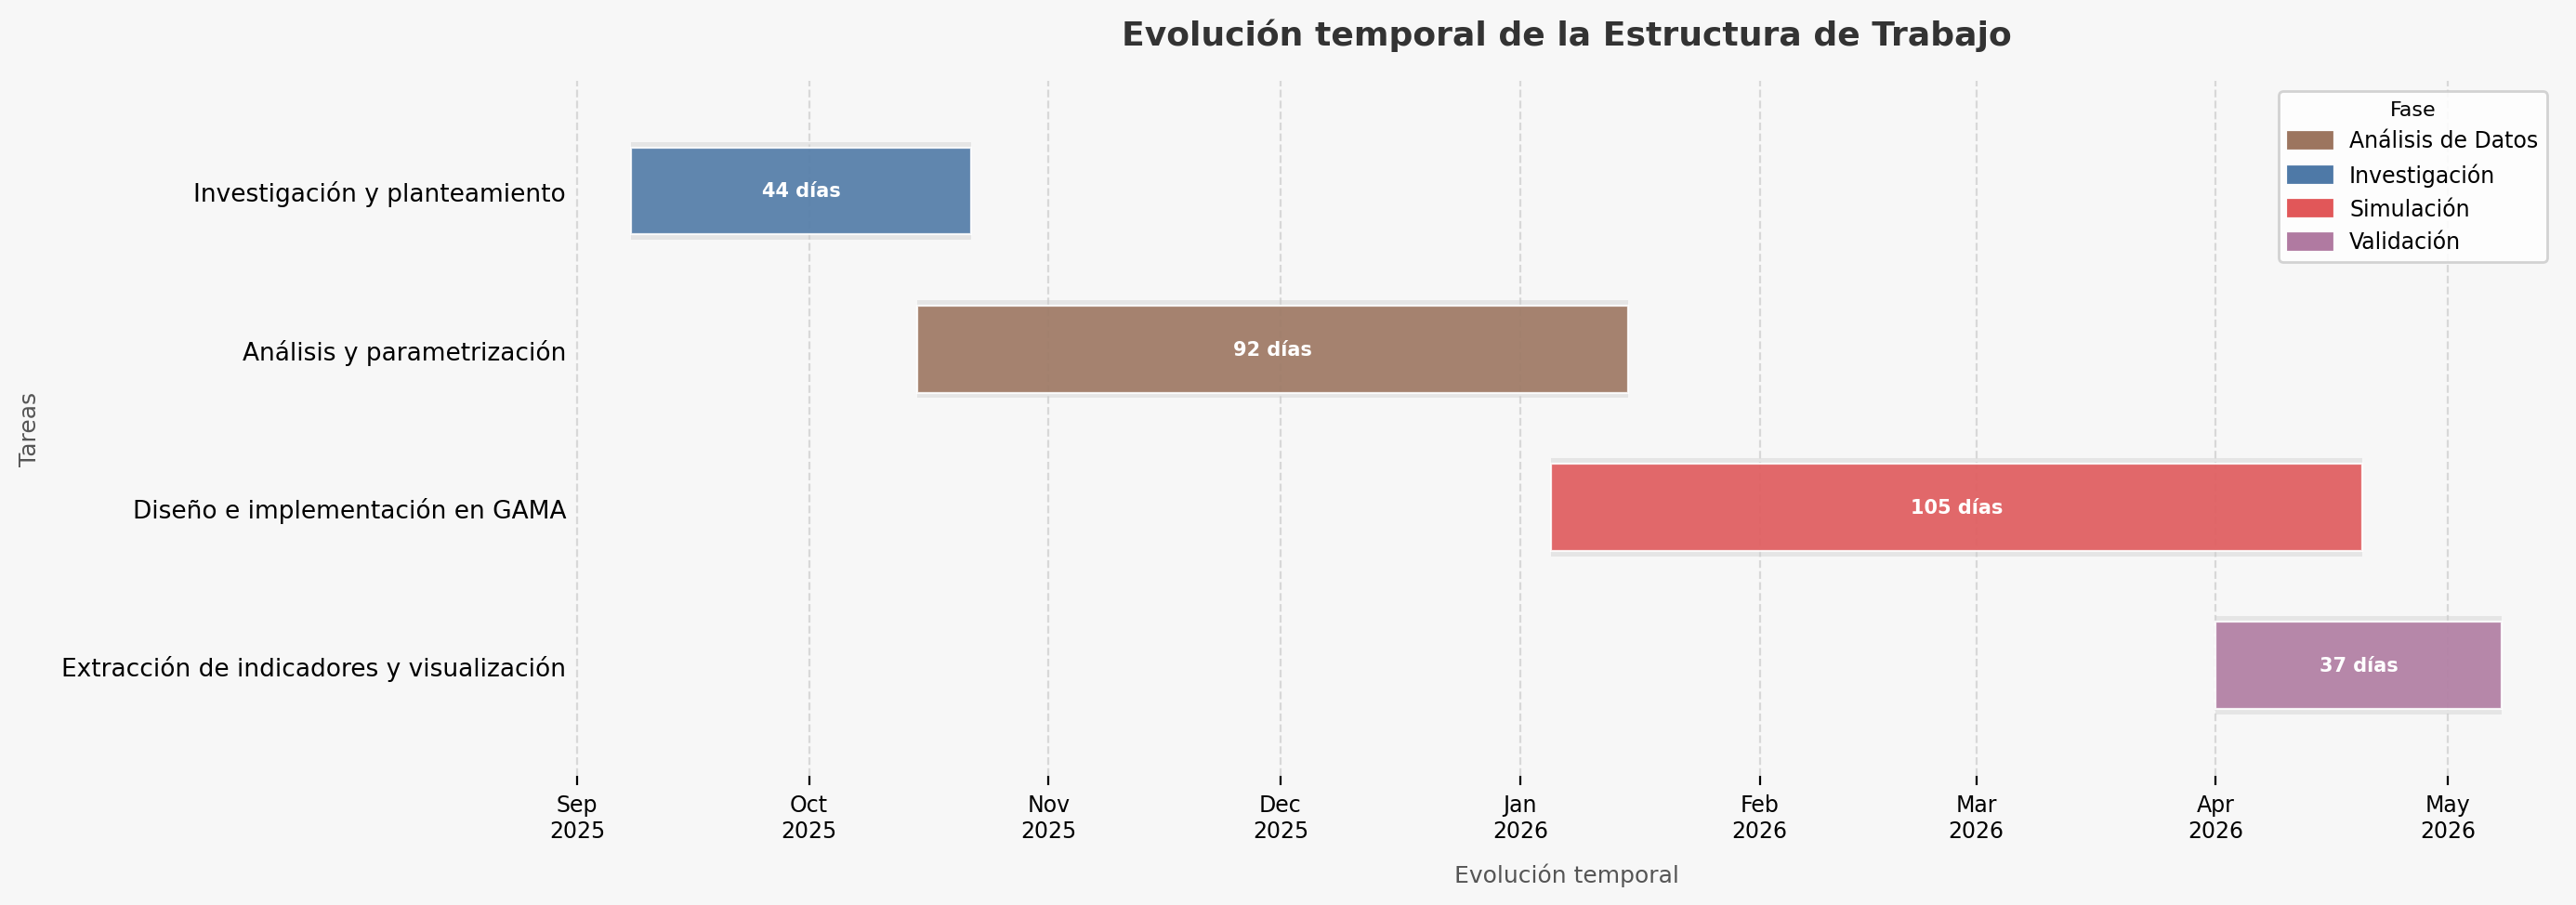
\includegraphics[width=0.9\textwidth,height=0.5\textheight]{imagenes/gantt_chart.png}
\caption{Diagrama de Gantt explicativo relativo a las distintas fases del desarrollo}
\par\vspace{4pt}{\footnotesize Fuente: Elaboración propia.}
\label{fig:gantt_diagram}
\end{figure}

\end{landscape}
\afterpage{
    \null
    \thispagestyle{plain}
}

\section{Herramientas Utilizadas}
En esta sección se exponen las distintas herramientas utilizadas para la construcción del sistema, junto a una breve explicación de su peso en ella.


\begin{itemize}


\item \textbf{GAMA}:
Usada en el desarrollo del sistema multi-agente, facilita la implementación del estándar de comunicaciones FIPA~\cite{fipa2002acl} y la inclusión de mapas geoespaciales. 

\item \textbf{Jupyter Notebook}\footnote{\url{https://jupyter.org} (accedido: 9 de mayo de 2026).}:
Herramienta usada con kernel de \textit{Python} para el análisis de los datos de operación de la línea a simular. Facilita la visualización de resultados, el análisis exploratorio de datos o la construcción de modelos estadísticos. Con  su estructura de celdas \enquote{markdown} y sus celdas de código, mejora la lectura y la explicabilidad de los procesos que se realizan en cada documento \enquote{ipynb} (formato de cuadernos Jupyter).

\item \textbf{QGIS}\footnote{\url{https://qgis.org} (accedido: 9 de mayo de 2026).}:
Necesaria para la conversión de GeoJSON (Formato basado en JSON con especificación concreta de parámetros para representación geográfica de los datos) a archivo ESRI shapefile (formato estándar de representación vectorial de datos geoespaciales) . Usada para la carga en el simulador de los datos de la ruta y de la ubicación de las paradas.

\item \textbf{Node.js}\footnote{\url{https://nodejs.org} (accedido: 9 de mayo de 2026).}:
Framework de desarrollo web utilizado para el despliegue de la herramienta en \textit{local}. Permite la creación de una arquitectura cliente/servidor que permita la conexión entre acciones o deseos del usuario en el navegador y su correspondiente cambio en la máquina anfitriona. Facilita la visualización de las simulaciones o el lanzamiento de nuevas.

\item \textbf{Docker}\footnote{\url{https://www.docker.com} (accedido: 9 de mayo de 2026).}:
Usado para la estandarización y aislamiento de procesos, facilitando el uso global del sistema. Utilizado para el despliegue de un contenedor encargado de la ejecución del programa completo, emulando un \enquote{gemelo digital} con las características del ordenador utilizado para el desarrollo. Gracias a esta herramienta, se permite ejecutar simulaciones en entornos sin la plataforma de desarrollo de agentes instalada.

\item \textbf{Python}\footnote{\url{https://www.python.org} (accedido: 9 de mayo de 2026).}:
Lenguaje de programación usado para la extracción de métricas de rendimiento de las distintas simulaciones. Sus librerías diseñadas para análisis de datos sobre grandes volúmenes como puede ser el caso de \textit{pandas} o generación de gráficas concretas con \textit{matplotlib} permiten generar estas KPIs con mayor facilidad.

\end{itemize}

Sobre las herramientas físicas utilizadas, se ha dispuesto de un portátil MSI Modern 15 C13M-273XES, 
modelo con 16 núcleos lógicos, 32GB RAM DDR4 y almacenamiento NVMe. Esta información, junto a detalles sobre presupuesto, 
se expanden en el capítulo \ref{chapter:budget}, pero cabe ser destacada por su relación a las herramientas usadas 
y su interés en la interpretación a nivel de tiempo en la fase de \textbf{Diseño
e implementación}, así como en la relativa a \textbf{Extracción de indicadores y visualización}.

Todo el desarrollo del trabajo se ha realizado sobre el sistema operativo Ubuntu 24.04 LTS, distribución 
de Linux basada en Debian. Esta elección de Sistema Operativo, sumado al conjunto de herramientas utilizadas,
 constituye un sistema de \textbf{código abierto} en su totalidad. Esto permite un sistema transparente y reproducible, 
 sin dependencia de licencias comerciales.

\chapter{Análisis de los datos}\label{chapter:param_analisys}
En este capítulo se describe el proceso de análisis y procesado de los datos otorgados por la EMT.
Se ha dividido en tres etapas: \textbf{Limpieza y Preparación}, \textbf{Estudio y Gaussianidad} y \textbf{Preparación para Simulador}.


\section{Limpieza y preparación}
Esta sección detalla los distintos procedimientos seguidos en una primera fase iniciada tras la recepción
de los datos provenientes de la EMT. Podemos distinguir dos tipos de datos principalmente:
Datos Geoespaciales y Datos de Operación.



\subsection{Datos geoespaciales}
Estos datos se corresponden con elementos públicos obtenidos del \textbf{EMT Open Data Portal}\footnote{
\url{https://datos.emtmadrid.es/} (accedido: 9 de mayo de 2026)}, una iniciativa
de la entidad que busca reforzar su compromiso con la transparencia y la colaboración para la mejoría
en la gestión~\cite{balaguer2018}. Si bien el simulador no necesita la exacta localización de las 
paradas o de la ruta en cuestión, estos datos permiten una mejor visualización de cara a la construcción
del modelo. Además, guardan información del orden y código numérico de las paradas, por lo que
se impulsó su integración y tratamiento.


Dichos datos se encuentran en formato GeoJSON, un estándar dentro del ámbito geoespacial. No obstante,
debido a la ubicación de estos dentro de un fichero de extensión \enquote{CSV}, se encuentran
mal formateados, presentando comillas simples \enquote{' '} en vez de comillas dobles 
\enquote{\char`\"  "}, y juntando ambos sentidos de la ruta dentro de la misma celda.

Para subsanar esto, se recurre a un script de \textit{Python} encargado de modificar las celdas 
correspondientes a los datos geo, separando en dos ficheros distintos según sentido y cambiando las 
occurrencias de comillas simples por dobles. Por facilidad, además, se ramificaron según si se 
correspondian con referencias a la trayectoria de la línea, o a instancias de paradas. 
De esta forma, se obtienen de cada ruta cuatro archivos, dos por cada sentido, donde uno
contiene información de la topología de las uniones inter-parada, y el otro de los puntos referencia a 
las mismas.


Como se especifica con anterioridad, aparte de obtención y limpieza de los datos, por facilidad en La
implementación, estos pasaron por un proceso de transformación a formato \textit{ESRI shapefile}.
Para ello se usa la herramienta de código abierto \textbf{QGIS}. En la figura \ref{fig:qgis_converted}
se muestra como se visualizan los cuatro GeoJSON procesados y transformados a shapefile. Posteriormente,
en la figura \ref{fig:shapefile_gama} se muestran esos archivos shapefile ya dentro del
entorno de trabajo de la plataforma de agentes GAMA.



\begin{figure}[H]
 \centering
    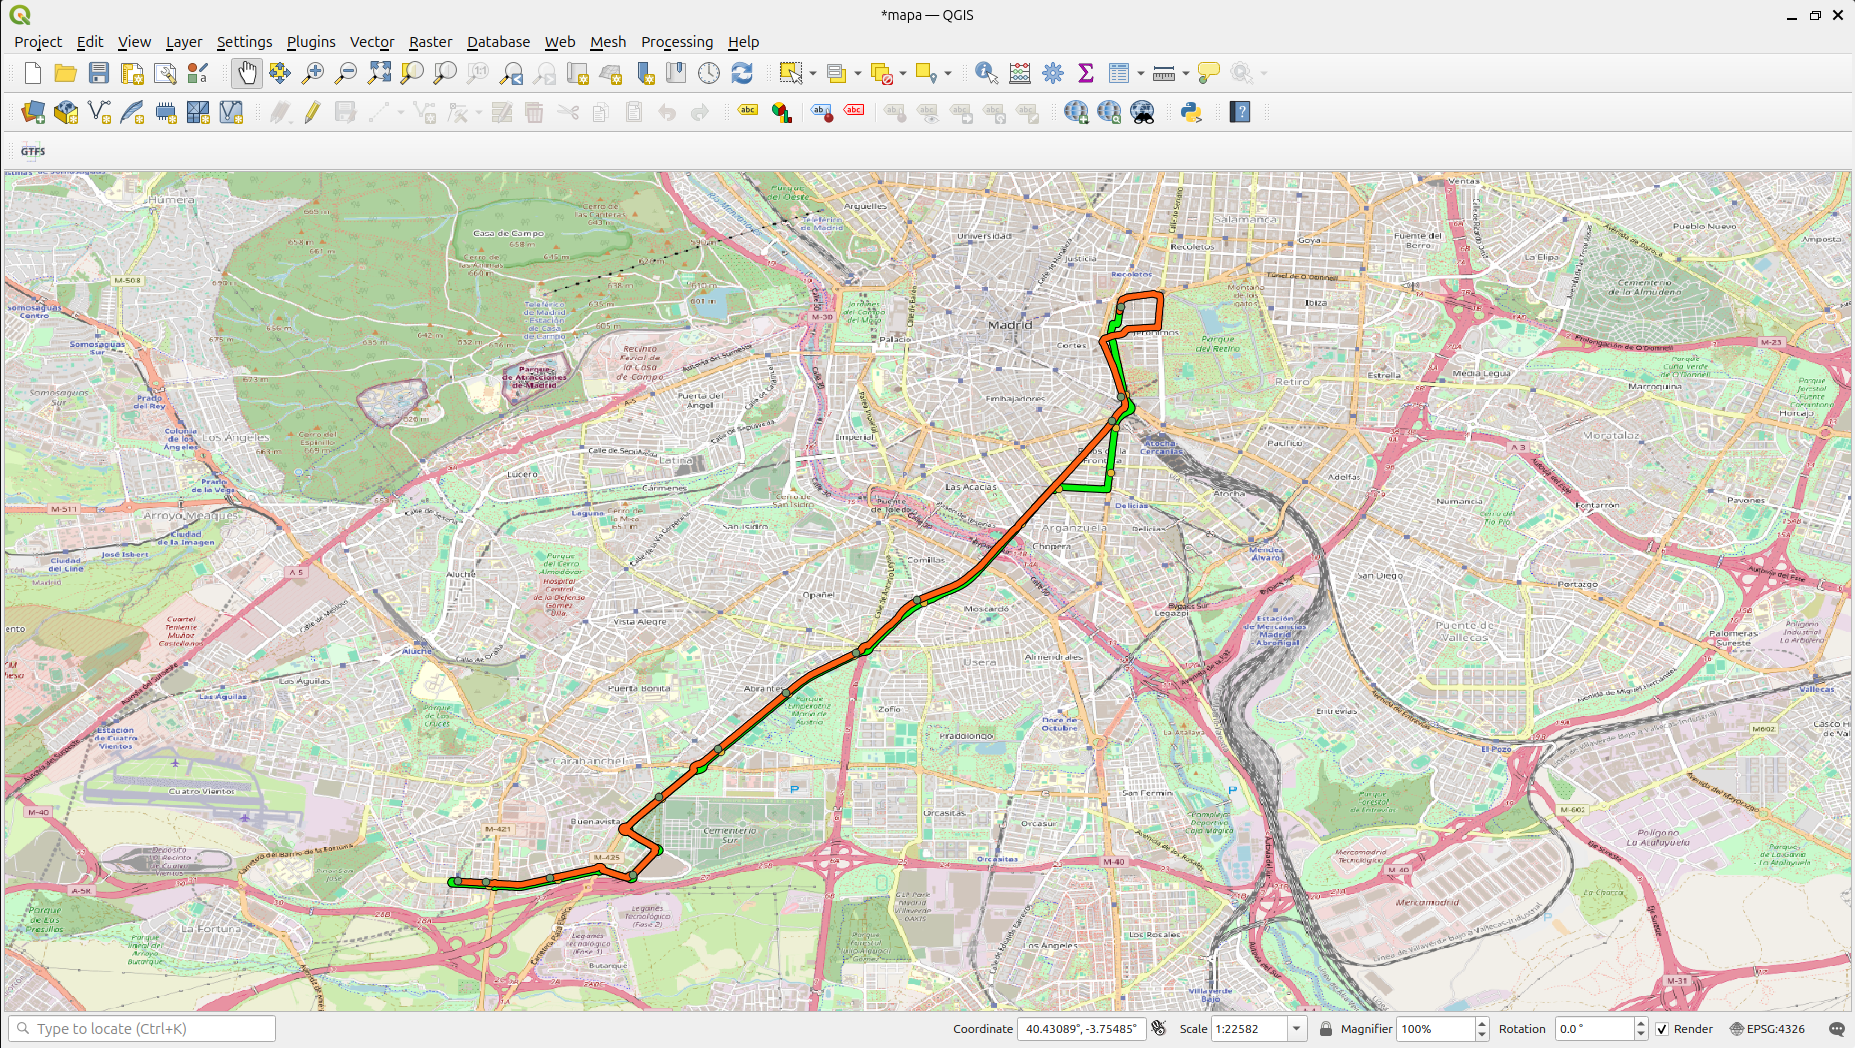
\includegraphics[width=\textwidth]{imagenes/qgis_capture_e01_converted.png}
\caption{Visualización en QGIS del mapa geoespacial convertido a shapefile}
\par\vspace{4pt}{\footnotesize Fuente: elaboración propia.}
\label{fig:qgis_converted}
\end{figure}


\begin{figure}[H]
 \centering
    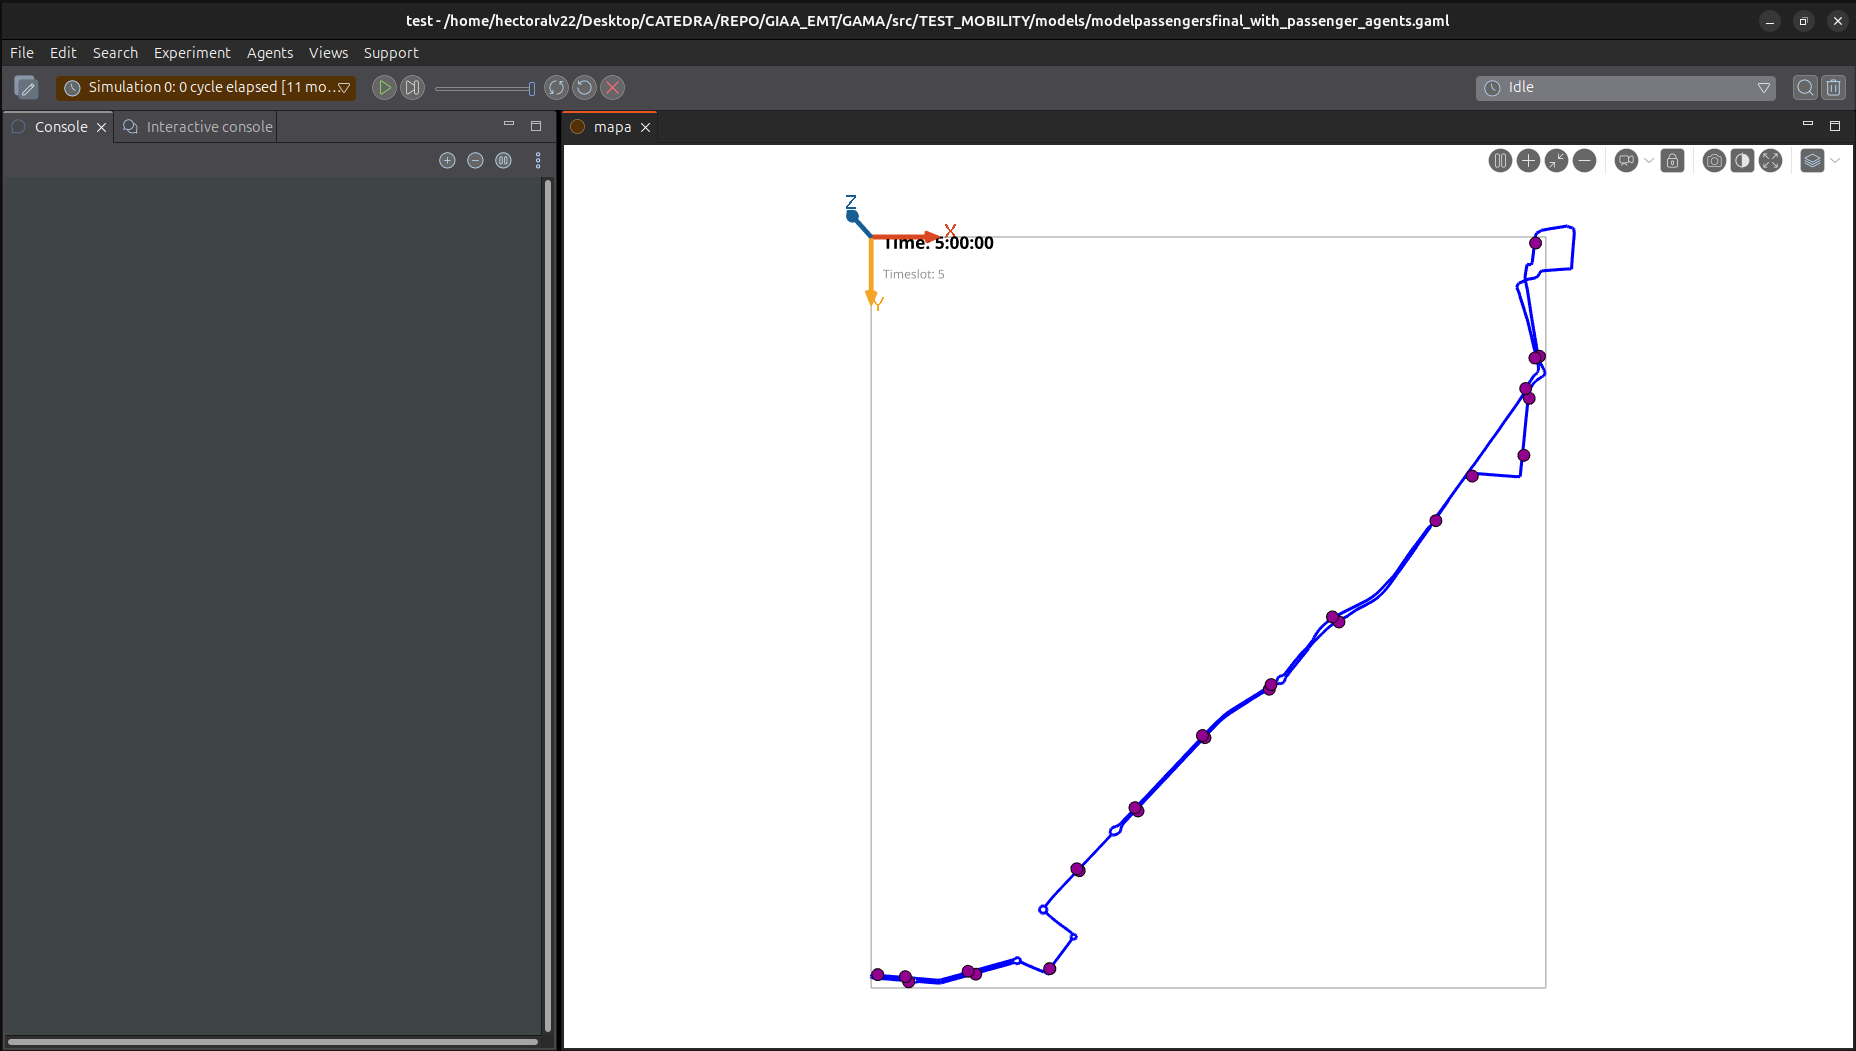
\includegraphics[width=\textwidth]{imagenes/gama_shapefiles.png}
\caption{Visualización en GAMA de los shapefile transformados}
\par\vspace{4pt}{\footnotesize Fuente: elaboración propia.}
\label{fig:shapefile_gama}
\end{figure}




\subsection{Datos de Operación}

Hablar de como se trabajaron los datos. Como se obtenian las tablas con  las consultas preparadas por stopcode, como se tuvo que limpiar valores negativos o anómalos, y explicar posibles discrepancias en primera y ultimas paradas debido(palabras de la emt quizas no se deba poner, que a veces los datos de inicio/fin estan falseados debido a que los conductores registran mal inicio/fin de viaje.

Los datos de operación representan la base empírica sobre la que se asienta el simulador.
Su tratamiento supuso el inicio formal de la fase dos del proyecto \textbf{Analisis y Parametrización},
debido a que la necesidad de la EMT  de preparar la base de datos en un servidor dedicado incluyendo el pipeline 
que alimenta diariamente los datos. Los geoespaciales por su parte, al ser de acceso público, se pueden tratar
sin la necesidad de preparación por parte de la empresa.

En la figura \ref{caption:relational_model} se puede ver el esquema relacional de la base de datos. Es un
modelo sencillo compuesto por dos tablas, Master y Transaccional, relacionadas por TripId,
identificador único de cada viaje. De esta forma, cada salida de cabecera representa una instancia de 
la tabla Master, mientras que cada llegada al resto de paradas de la ruta supone una entrada
de la tabla transaccional, identificada por el mismo TripId y el código de parada.


\begin{figure}[H]
 \centering
    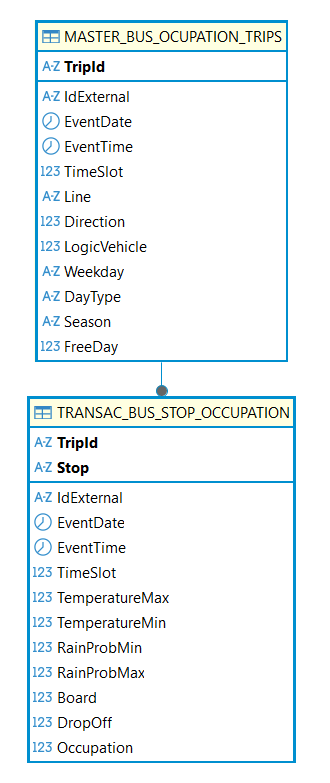
\includegraphics[width=0.5\textwidth]{imagenes/image_tables_diagram.png}
\caption{Modelo Master:Transaccional de la base de datos}
\par\vspace{4pt}{\footnotesize Fuente: Documento facilitado por la EMT.}
\label{caption:relational_model}
\end{figure}

\begin{lstlisting}[language=SQL, caption={Datos totales de una parada}]
SELECT mbot.*, tbso.*
FROM UCIII.Transport.MASTER_BUS_OCUPATION_TRIPS mbot
JOIN UCIII.Transport.TRANSAC_BUS_STOP_OCCUPATION tbso
    ON tbso.TripId = mbot.TripId
\end{lstlisting}
\par\vspace{4pt}{\footnotesize Fuente: Documento Facilitado por la EMT.}



\chapter{Diseño de la simulación}\label{chapter:simulation_design}



\textbf{Aqui basicamente tengo que dividirlo en varias partes. Primeramente hablar del diseño y la eleccion como 
de la arquitectura de los agentes, el por qué de cada protocolo de comunicacion, como funciona un flujo de un 
autobus llegando a la parada, el tema del suavizado de cambios entre valores de franjas, etc.
Tambien discutir sobre los dos modelos existentes, que el que incluye pasajeros puede ser considerado más 
"de agentes" por su comportamiento mas parecido a la realidad, con pasajeros que piden bajar, buses que rechazan 
subir más gente, y el otro que es más orientado a simulaciones rápidas(15 mins) pero que ambos generan mismos
resultados sobre el papel. Puedo tmb meter una ontologia? Para mostrar un poco la arquitectura de los distintos
elementos que componen cada simulacion. Hablar tambien de como se recogen los resultados, los logs etc}



%No se si será asi el titulo o no
\chapter{Casos de Aplicación}\label{chapter:application_cases}
Este capítulo recoge los resultados obtenidos con el sistema desarrollado, abarcando tanto la validación del simulador frente a los datos
operativos reales como la experimentación mediante modificación paramétrica de los escenarios. Para ello, se estructura en cuatro secciones.
La primera, a modo introductorio, presenta el funcionamiento operativo del sistema completo. La segunda presenta los distintos indicadores de
rendimiento (KPIs) considerados y su visualización para cada solución. La tercera aborda la validación operativa del simulador y la comparativa
entre las dos soluciones presentadas en el capítulo anterior. Por último, la cuarta cubre la experimentación mediante modificación paramétrica
del sistema, contrastando los resultados obtenidos frente a las hipótesis planteadas.

\section{Funcionamiento operativo del sistema final}\label{sec:general_behaviour}
Si bien el núcleo del presente trabajo lo constituye el simulador multiagente desarrollado sobre GAMA, su explotación práctica requiere de un medio
que permita a un usuario no especializado configurar, lanzar y consultar simulaciones sin interactuar directamente con la plataforma.
Con este propósito, y conforme a los requisitos definidos en el marco de la colaboración con la EMT~(recogidos en el anexo~\ref{anex:requirements}),
el sistema final incorpora una interfaz web que actúa como capa intermedia entre el usuario y el simulador. Cabe destacar que dicha interfaz no 
constituye un objetivo de investigación en sí misma, sino el instrumento mediante el cual se orquestan los lanzamientos y se visualizan los 
resultados que se presentan a lo largo de este capítulo.

La interfaz centraliza tres funciones: la parametrización de los escenarios de simulación, el lanzamiento y almacenamiento de las ejecuciones,
y la visualización de los indicadores de rendimiento resultantes. Con el fin de garantizar la reproducibilidad del despliegue y eliminar
dependencias del sistema anfitrión, el conjunto completo se distribuye sobre una imagen de \textit{Docker}, de modo que simulador, interfaz y
persistencia de resultados se ejecutan de forma autocontenida.

Los resultados presentados en las secciones posteriores derivan tanto de figuras como de instantáneas de dicha interfaz. La exposición acerca
de cómo se visualiza cada indicador de forma individual se presenta a continuación en la siguiente sección.

\section{Estructura y visualización de los KPIs}\label{sec:kpi_visualization}

Manteniendo la estructura de métricas presentada en la sección~\ref{sec:kpi_extraction}, se presenta para cada categoría su
correspondiente indicador mostrado en la interfaz. Cabe destacar que tanto las figuras generadas como los valores relativos a cada 
indicador se computan una única vez al finalizar cada simulación, y no bajo demanda en el momento de la consulta. Este cómputo se 
realiza para todas las combinaciones de filtrado posibles, por lo que el usuario final experimentará tiempos de respuesta prácticamente
inmediatos en el muestreo de resultados. 

De forma previa a la presentación de cada métrica, resulta imperioso remarcar que, con el objetivo de sintetizar alertas visuales
para la detección de posibles puntos críticos, donde se estén dando resultados anómalos, se ha dispuesto de un sistema heurístico basado
en umbrales que, mediante clasificación por colores, permita al usuario identificar dichos puntos para una rápida exploración de estos.
Dicho sistema resulta implementado tanto en las \textbf{métricas a nivel de ruta} como en las \textbf{métricas a nivel de autobús}. En cada apartado
correspondiente se expande la información relevante sobre los umbrales determinados.









\subsection{Métricas a nivel general}

\subsection{Métricas a nivel de ruta}

\subsection{Métricas a nivel de autobús}


% \subsection{Sistema de catalogación de resultados}
% Resulta importante exponer el \textbf{criterio de identificación de resultados destacables} implementado para la interfaz.

% Este consiste en una clasificación por colores según distintos parámetros, que, a modo de nivel de alerta visual, permiten identificar
% posibles puntos donde se estén dando resultados anómalos. Para ello, se especifican valores a modo de frontera para cada uno de los cuatro
% campos a estudiar.

% Concretamente:

% \begin{enumerate}
%     \item \textit{Valor de regularidad}:

%     Se establece el valor~\textbf{80} como valor mínimo requerido para no activar este indicador.

%     \item \textit{Porcentaje de simulaciones con retraso}:
    
%     Se activa este indicador siempre que el indicador relativo a este campo para cada expedición de un un autobús muestre un porcentaje
%     de réplicas con retraso \textbf{superior al 20\%}.

%     \item \textit{Tiempo medio de retraso en la salida}:
    
%     Por otra parte y relativo al retraso en la salida, este indicador se activará siempre que 
% \end{enumerate}


% const ALERT_THRESHOLDS = {
%   regularity_min:  80,   // Regularity_value < 80
%   delay_pct_max:   20,   // Percentage_sims_delay_departure > 20%
%   delay_secs_max: 300,   // Mean_Minutes_departure_delay > 300s (5 min)
%   occupation_max:  60,   // Mean_Occupation_Percentage > 60%
% };



\section{Validación operativa y comparativa de soluciones}\label{sec:validation}



\section{Experimentación paramétrica}\label{sec:experiments}







%%%%%%%%NO SE ME PUEDEN OLVIDAR :)
\chapter{Marco Regulador}
Este capítulo cubre 




\section{Protección de datos y privacidad (RGPD)}

\section{Licencias de software y herramientas de terceros}

\section{Uso de la información del sector público (Open data)}

\section{Propiedad intelectual del proyecto}

\section{Ética profesional}



\textit{ \textbf{Posible opción}
El desarrollo de este Trabajo de Fin de Grado se ha guiado por los principios fundamentales del Código de Ética y
Práctica Profesional de Ingeniería de Software (ACM/IEEE). Desde una perspectiva deontológica, la ingeniería 
informática no consiste únicamente en la resolución técnica de problemas, sino en la aplicación del conocimiento 
empírico para orientar la tecnología hacia el bien común. En este contexto, el simulador diseñado busca un beneficio 
social tangible e inmediato: proporcionar a la Empresa Municipal de Transportes una herramienta objetiva para 
optimizar las dotaciones programadas, mejorando así la eficiencia y sostenibilidad de la movilidad urbana. Si bien 
es inherente a la ingeniería de software que los sistemas complejos pueden generar consecuencias operativas o sociales 
imprevisibles, la responsabilidad ética del diseño se ha salvaguardado mediante la aplicación de medidas rigurosas y 
estándares contrastados de la profesión. El uso de validaciones estadísticas exhaustivas y metodologías robustas como 
la simulación de Monte Carlo garantiza los más altos niveles de calidad técnica y fiabilidad, limitando los riesgos 
derivados de la puesta en producción del software.
Asimismo, el compromiso ético del proyecto trasciende el estricto cumplimiento legal impuesto por normativas de
privacidad como el RGPD. En el ámbito de la automatización y el diseño algorítmico, se ha prestado especial atención a
la mitigación de sesgos computacionales que pudieran derivar en discriminación o en un análisis deficiente de la
calidad del servicio. Por ello, el sistema modela el comportamiento de la red basándose de forma estricta en datos
operacionales empíricos y agregados. Al descartar explícitamente dotar a los agentes simulados de capacidades
deliberativas arbitrarias sin fundamento en los datos, se evita la introducción de sesgos de confirmación o decisiones
algorítmicas opacas. De este modo, se asegura que la herramienta evalúe el rendimiento del transporte público de manera
transparente y equitativa, respetando el interés general de la ciudadanía y evitando cualquier discriminación en la
planificación de los recursos urbanos.}

\chapter{Entorno socio-económico}\label{chapter:budget}
\section{Presupuesto}


\section{Impacto socio-económico}


\chapter{Limitaciones y trabajos futuros}\label{chapter:future_works}
\textbf{Hablar de la funcion constante  del ratio de generacion de psajeros}
\chapter{Conclusión}
\section{Resumen del trabajo realizado}
El trabajo expuesto a lo largo de este documento resulta de la consecución de cuatro fases concretas.

Conceptualmente se inicia con la contextualización del problema, donde se introduce la idea de buscar la forma de simular
la operación de una línea de autobús a lo largo de un día de servicio. Para ello, previa investigación de literatura existente,
se escoge el paradigma multi-agente, debido a las características del entorno dinámicas y complejas, junto a la capacidad de evolución
que presenta.

Una vez queda definido el objetivo, se empieza a trabajar sobre el conjunto de datos otorgado por la EMT. Durante esta fase, se acota
el alcance del simulador debido a distintas características observadas, como la exclusión de fines de semana o de días con gratuidad.
Debido también a la estructura de los datos, se caracteriza estadísticamente mediante distribuciones tanto valores comparativos 
de ocupación, como la carga y descarga de pasajeros, siendo estos últimos los principales parámetros estocásticos del sistema multi-agente.

Con los datos estudiados y el objetivo contextualizado, se inicia la fase de construcción del sistema. En esta fase se opta por el
desarrollo de dos sistemas paralelos, que se diferencian por la caracterización en uno de ellos de los pasajeros como agentes, pero
con el objetivo de que ambos sean plenamente funcionales bajo el escenario a modelar. En esta fase se modela la arquitectura
en la plataforma de diseño de agentes GAMA, y se implementan conceptos como la reconstrucción lineal conservativa, para incorporar
la tendencia en la generación de pasajeros, se diseñan protocolos de comunicación basados en los estándares FIPA, 
o se resuelven conflictos como la abstracción de la inferencia de bajada de pasajeros mediante acciones del entorno, extrayendo
estas capacidades de los agentes.

Por último, y en concordancia con lo establecido en los requisitos del sistema, se construye
una interfaz que facilita el lanzamiento y la visualización de las simulaciones, permitiendo
abordar la validación de forma más ágil.

Dicha validación muestra que el simulador reproduce la operativa de la línea con un sesgo
medio en torno a los dos pasajeros y una sobredispersión que crece a lo largo del recorrido,
magnitudes ambas caracterizadas y documentadas. Se identifica asimismo que el modelado de
descensos como eventos independientes restringe la validez del sistema al escenario base,
excluyendo el análisis de configuraciones alternativas de servicio.

\section{Satisfacción de objetivos}
Para el presente trabajo se establece un objetivo principal y tres objetivos secundarios. A lo largo del documento se ha discutido,
especialmente en el capítulo correspondiente a la validación y resultados (véase capítulo~\ref{chapter:application_cases}), la completitud
de los distintos objetivos. A continuación, para cada uno se formaliza y se discute en profundidad su grado de conformidad alcanzado.

\subsection{Satisfacción del objetivo principal del trabajo}
Este objetivo concretamente es \textbf{determinar en qué medida un sistema multi-agente parametrizado a partir de datos reales
es capaz de reproducir la operativa de una línea de autobús urbano.} Tras la construcción
y evaluación del sistema multi-agente para las dos implementaciones, se puede concluir que el objetivo principal del trabajo
resulta satisfecho, ya que se constata que, pese a la discusión relativa al sesgo y a la sobredispersión, el sistema es capaz
de capturar el comportamiento general de la línea de estudio para los días laborables y estudiar, en base a los indicadores
de rendimiento obtenidos, la capacidad de absorción de la demanda por parte de la operativa de servicio promedio.

\subsection{Satisfacción de los objetivos secundarios}

En cuanto a los objetivos secundarios, el primero de ellos, \textbf{caracterizar estadísticamente los datos operacionales de la línea},
se satisface mediante el análisis
recogido en el capítulo~\ref{chapter:param_analisys}. Los datos operacionales cedidos por la
EMT han sido depurados y caracterizados estadísticamente, ajustando distribuciones de
probabilidad sobre los valores de ocupación, embarque y descenso para cada combinación de
parada y franja horaria, con la selección de familia realizada mediante criterios de bondad
de ajuste y de información.

El segundo objetivo, \textbf{validar que ambas propuestas arquitectónicas generan resultados equivalentes},
queda igualmente cumplido. El contraste directo de los indicadores de
rendimiento generados por ambas soluciones, bajo idénticos parámetros de entrada, confirma que las dos propuestas arquitectónicas
producen resultados equivalentes. Se puede concluir entonces que tanto la representación agregada como la
representación basada en agentes pasajero individuales reproducen el comportamiento esperado.

Por último, el tercer objetivo, \textbf{proporcionar una herramienta que permita ejecutar, almacenar y visualizar de forma
interactiva las distintas simulaciones generadas por el sistema}, queda satisfecho mediante la construcción de la interfaz presentada
al inicio del capítulo~\ref{chapter:application_cases}, que unifica todos los requerimientos del objetivo.

\section{Conclusiones generales}
En un cómputo general, este trabajo de investigación se posiciona como la fase inicial o de validación de un proyecto colaborativo
entre entidades públicas, cuyo objetivo último es servir como herramienta para analizar y mejorar el servicio de autobuses 
urbanos.

El trabajo realizado asienta la base sobre la que evolucionar el sistema hacia dicho
objetivo. La elección del paradigma multi-agente permite un escalado posterior hacia
arquitecturas deliberativas sin alterar el esqueleto del modelo. La interfaz implementada
facilita el lanzamiento, almacenamiento y visualización de escenarios. Y el análisis de los
datos operacionales, si bien constituye el origen de la principal limitación identificada,
delimita con precisión qué aspectos del servicio resultan reproducibles y con qué grado de
fidelidad.

Cabe destacar que la validación del sistema no se ha limitado a demostrar el acuerdo entre
lo simulado y lo observado, sino que ha perseguido caracterizar dónde falla el modelo y por
qué mecanismo. Es dicha caracterización, más que el acuerdo en sí, la que permite establecer
sobre qué preguntas puede el simulador aportar respuesta y cuáles quedan condicionadas a
desarrollos posteriores.

%----------
%	BIBLIOGRAFÍA
%----------	

%\nocite{*} % Si quieres que aparezcan en la bibliografía todos los documentos que la componen (también los que no estén citados en el texto) descomenta está línea

\clearpage
\addcontentsline{toc}{chapter}{Bibliografía}
\setquotestyle[english]{british} % Cambiamos el tipo de cita porque en el estilo IEEE se usan las comillas inglesas.
\printbibliography



%----------
%	ANEXOS
%----------	

% Si tu trabajo incluye anexos, puedes descomentar las siguientes líneas

% --- Justo al terminar el cuerpo principal, ANTES del primer anexo ---
\appendix
\renewcommand{\appendixname}{Anexo}   % "Anexo A" en lugar de "Apéndice A"

\titleformat{\chapter}[block]
{\large\bfseries\filcenter}
{\MakeUppercase{\appendixname}\ \thechapter.}
{5pt}
{\MakeUppercase}
{}

\chapter{Especificación de Requisitos del Sistema}\label{anex:requirements}
% ----------------------------------------------------------
%  Macro \requisito
%  Las fichas NO aparecen en el \listoftables.
%
%  Uso:
%    \requisito{ID}{Nombre}{Tipo}{Prioridad}{Fuente}
%              {Descripcion}{Justificacion}{Dependencias}
%              {Verificacion}
%
%  Tipo:      RF | RNF | RD
%  Prioridad: Must | Should | Could   (MoSCoW)
%  Metodo:    T=Test  I=Inspeccion  A=Analisis  D=Demostracion
% ----------------------------------------------------------
 



\newcommand{\requisito}[9]{%
  \vspace{6pt}
  \noindent\small\textbf{#1 \textemdash\ \MakeUppercase{#2}}
  \vspace{2pt}
 
  \noindent\small
  \begin{tabular}{|p{3.5cm}|p{9.5cm}|}
  \hline
  \textbf{Identificador}      & #1 \\ \hline
  \textbf{Nombre}             & #2 \\ \hline
  \textbf{Tipo}               & #3 \\ \hline
  \textbf{Prioridad}          & #4 \\ \hline
  \textbf{Fuente}             & #5 \\ \hline
  \textbf{Descripción}   & #6 \\ \hline
  \textbf{Justificación} & #7 \\ \hline
  \textbf{Dependencias}       & #8 \\ \hline
  \textbf{Verificación}  & #9 \\ \hline
  \end{tabular}
  \vspace{8pt}
}


 
% -------------------------------------------------------
\section*{A.1\quad Introducción}
% -------------------------------------------------------
 
[Texto introductorio aquí]
 
% -------------------------------------------------------
\section*{A.2\quad Requisitos Funcionales}
% -------------------------------------------------------
 
\requisito
  {RF-01}
  {[Nombre corto del requisito]}
  {Funcional}
  {Must}
  {[Fuente: tutor, normativa EMT, IEEE\,29148, etc.]}
  {[Descripción completa, precisa y verificable del comportamiento requerido.]}
  {[Por qué este requisito es necesario.]}
  {RF-XX, RNF-XX  o Ninguna}
  {[Como se comprueba que el requisito se cumple \quad Metodo T/I/A/D ]}


\requisito
  {RNF-01}%Identificador
  {Fidelidad descriptiva}%Nombre
  {RNF}%Tipo
  {Must}%Prioridad
  {EMT}%Fuente
  {El modelo de simulación deberá reproducir la operación de la línea de modo que las distribuciones de sus métricas de 
  salida (intervalos de paso, tiempos de parada, ocupación y subidas/bajadas por parada y franja horaria) sean 
  estadísticamente consistentes con los datos de referencia proporcionados por la EMT, dentro de una tolerancia 
  previamente definida.}%Descripción
  {La EMT requiere un modelo de carácter descriptivo, fiel a los datos observados, sin introducir comportamientos 
  inventados ni desviaciones respecto de la operación real registrada. Este requisito constituye la restricción de 
  validez que gobierna el paradigma de modelado adoptado.}%Justificación
  {---}%Dependencias
  {A --- Pruebas de bondad de ajuste (Kolmogórov---Smirnov / $\chi^2$) entre las distribuciones simuladas y las 
  observadas sobre el conjunto de 1000 réplicas.}%Verificación
 
 
% ---------- Requisitos funcionales: comportamiento del autobús ----------
 
\requisito
  {RF-01}%Identificador
  {Salidas según horario programado}%Nombre
  {RF}%Tipo
  {Must}%Prioridad
  {EMT}%Fuente
  {Cada agente autobús deberá iniciar su recorrido desde la cabecera en los instantes de salida establecidos en el 
  horario oficial de la EMT.}%Descripción
  {La planificación temporal del servicio forma parte de los datos operativos reales y debe respetarse para garantizar 
  la fidelidad descriptiva (RNF-01).}%Justificación
  {RNF-01}%Dependencias
  {I --- Inspección de las trazas de ejecución frente al horario de referencia.}%Verificación
 
\requisito
  {RF-02}%Identificador
  {Secuencia fija de paradas}%Nombre
  {RF}%Tipo
  {Must}%Prioridad
  {EMT}%Fuente
  {Cada agente autobús deberá recorrer la secuencia ordenada y fija de paradas correspondiente a su ruta y 
  sentido asignados.}%Descripción
  {El trazado de la línea es un dato fijo de la operación real; no se contempla ninguna variación de itinerario 
  (véase RD-01).}%Justificación
  {RNF-01, RD-01}%Dependencias
  {I --- Inspección de las trazas de paso por las paradas.}%Verificación
 
\requisito
  {RF-03}%Identificador
  {Tiempo entre paradas empírico}%Nombre
  {RF}%Tipo
  {Must}%Prioridad
  {EMT}%Fuente
  {El tiempo de viaje entre paradas consecutivas deberá obtenerse por muestreo de la distribución empírica 
  de tiempos entre paradas correspondiente a la parada, el sentido y la franja horaria.}%Descripción
  {Los tiempos de desplazamiento se derivan de los datos registrados, evitando cualquier valor inventado 
  (RNF-01, RD-03).}%Justificación
  {RNF-01, RD-03}%Dependencias
  {A --- Comparación estadística entre la distribución de tiempos simulados y la empírica.}%Verificación
 
\requisito
  {RF-04}%Identificador
  {Tiempo de parada derivado de la demanda}%Nombre
  {RF}%Tipo
  {Must}%Prioridad
  {EMT}%Fuente
  {El tiempo de permanencia del autobús en cada parada deberá derivarse del número de subidas y bajadas 
  procesadas en dicha parada.}%Descripción
  {El tiempo de parada es una consecuencia directa de la demanda atendida; su cálculo a partir de subidas y 
  bajadas asegura la coherencia con la operación real.}%Justificación
  {RF-05, RF-06}%Dependencias
  {T --- Prueba funcional sobre el cálculo del tiempo de espera en función de subidas y bajadas.}%Verificación
 
 
% ---------- Requisitos funcionales: alineamiento empírico de subidas/bajadas ----------
 
\requisito
  {RF-05}%Identificador
  {Subidas conforme a la distribución empírica}%Nombre
  {RF}%Tipo
  {Must}%Prioridad
  {EMT}%Fuente
  {Las subidas de viajeros generadas en cada parada deberán muestrearse a partir de la distribución empírica 
  de subidas correspondiente a la parada y la franja horaria.}%Descripción
  {La generación de demanda debe reproducir los volúmenes de subida observados (RNF-01).}%Justificación
  {RNF-01}%Dependencias
  {A --- Comparación de distribuciones entre las subidas simuladas y las observadas.}%Verificación
 
\requisito
  {RF-06}%Identificador
  {Bajadas conforme a la distribución empírica}%Nombre
  {RF}%Tipo
  {Must}%Prioridad
  {EMT}%Fuente
  {Las bajadas de viajeros en cada parada deberán reproducir la distribución empírica de bajadas correspondiente a la
   parada y la franja horaria. La selección de los viajeros que descienden se realiza mediante un mecanismo centralizado
    (\textit{invisible hand}) que marca el número de descensos muestreado de dicha distribución.}%Descripción
  {La EMT proporciona recuentos agregados de bajadas por parada y franja horaria, pero no datos de origen--destino
   individuales de los viajeros. En ausencia de dicha información, imponer las bajadas como una función a nivel de 
   sistema que reproduce la distribución medida es el único mecanismo coherente con RNF-01 sin vulnerar la prohibición 
   de comportamientos no fundamentados en datos (RD-03).}%Justificación
  {RNF-01, RD-03}%Dependencias
  {A --- Comparación de distribuciones entre las bajadas simuladas y las observadas.}%Verificación
 
\requisito
  {RF-07}%Identificador
  {Restricción de capacidad y subidas residuales}%Nombre
  {RF}%Tipo
  {Must}%Prioridad
  {EMT}%Fuente
  {La ocupación de cada autobús no deberá superar la capacidad máxima del vehículo; las subidas que excedan 
  dicha capacidad deberán registrarse como subidas residuales (no embarcadas).}%Descripción
  {La capacidad finita del vehículo es una restricción física real, y la cuantificación de la demanda no atendida 
  constituye una métrica relevante del análisis.}%Justificación
  {RF-05}%Dependencias
  {T --- Verificación del invariante de capacidad y del recuento de residuales sobre el conjunto de réplicas.}%Verificación
 
 
% ---------- Restricciones de diseño: prohibiciones que delimitan el modelo descriptivo ----------
 
\requisito
  {RD-01}%Identificador
  {Ausencia de reenrutamiento dinámico}%Nombre
  {RD}%Tipo
  {Must}%Prioridad
  {EMT}%Fuente
  {Los agentes autobús no deberán realizar reenrutamiento dinámico; la ruta permanecerá fija durante toda la 
  prestación del servicio.}%Descripción
  {La EMT exige reproducir la operación real sin desviaciones de itinerario; el reenrutamiento introduciría un 
  comportamiento no presente en los datos.}%Justificación
  {RNF-01}%Dependencias
  {I --- Inspección del modelo: ausencia de lógica de reenrutamiento.}%Verificación
 
\requisito
  {RD-02}%Identificador
  {Ausencia de comportamiento cooperativo o estratégico}%Nombre
  {RD}%Tipo
  {Must}%Prioridad
  {EMT}%Fuente
  {Los agentes no deberán exhibir comportamientos cooperativos, negociados o estratégicos más allá del 
  protocolo de subida y bajada fundamentado en los datos (sin coordinación entre autobuses, sin regulación de 
  intervalos ni peticiones de ayuda).}%Descripción
  {Cualquier conducta deliberativa o cooperativa constituiría un comportamiento inventado, ajeno al carácter descriptivo 
  del modelo y no validable frente a los datos de la EMT.}%Justificación
  {RNF-01}%Dependencias
  {I --- Inspección del modelo: ausencia de mecanismos de coordinación o negociación.}%Verificación
 
\requisito
  {RD-03}%Identificador
  {Comportamiento fundamentado únicamente en datos}%Nombre
  {RD}%Tipo
  {Must}%Prioridad
  {EMT}%Fuente
  {No deberá introducirse ningún comportamiento de los agentes que no sea derivable de los datos de referencia de 
  la EMT o calibrado contra ellos.}%Descripción
  {Constituye la expresión, como restricción de diseño, del mandato de fidelidad descriptiva (RNF-01): el modelo debe 
  limitarse a lo que los datos permiten fundamentar. RNF-01 y RD-03 son, por tanto, las dos formulaciones --- positiva y 
  restrictiva --- de un mismo requisito de la EMT.}%Justificación
  {RNF-01}%Dependencias
  {I --- Inspección y trazabilidad de cada comportamiento del modelo hasta su fuente de datos.}%Verificación






% =====================================================================
% REQUISITOS DEL SISTEMA — Simulador multiagente de la línea E01 (EMT Madrid)
%
% Convenciones:
%   - RF-XX  : requisitos funcionales (fuente principal: EMT Madrid)
%   - RD-XX  : restricciones/requisitos de diseño
%   - RNF-XX : requisitos no funcionales
%   - Prioridad: MoSCoW (Must / Should / Could)
%   - Verificación: método T = Prueba, I = Inspección, A = Análisis,
%                   D = Demostración
% =====================================================================

\subsection{Requisitos funcionales}

\requisito{RF-01}{Creación de simulaciones desde la interfaz web}
{Funcional}
{Must}
{EMT Madrid}
{El sistema debe permitir al usuario crear una nueva simulación desde la interfaz web, generando un directorio de trabajo versionado e identificado mediante marca temporal que aísle la configuración y los resultados de cada ejecución.}
{El personal técnico de la EMT debe poder preparar escenarios sin manipular ficheros ni ejecutar comandos manualmente, y cada escenario debe quedar aislado del resto para su posterior consulta.}
{---}
{Creación de una simulación desde la interfaz y comprobación del directorio generado. Método: D}

\requisito{RF-02}{Configuración de los parámetros del escenario}
{Funcional}
{Must}
{EMT Madrid}
{Antes del lanzamiento, el sistema debe permitir al usuario personalizar los parámetros operativos del escenario, incluyendo el tamaño y la composición de la flota, los horarios e intervalos entre expediciones y las distribuciones de subidas y bajadas por parada y franja horaria.}
{La utilidad del simulador para la EMT reside en evaluar escenarios operativos alternativos (más o menos autobuses, otras frecuencias, otras demandas) sin necesidad de modificar el modelo.}
{RF-01}
{Modificación de cada parámetro desde la interfaz y comprobación de su efecto en la simulación resultante. Método: T}

\requisito{RF-03}{Lanzamiento de simulaciones desde la interfaz web}
{Funcional}
{Must}
{EMT Madrid}
{El sistema debe permitir lanzar la ejecución de la simulación configurada desde la propia interfaz web, invocando de forma transparente el motor de simulación en modo desatendido.}
{Cierra el ciclo de uso autónomo por parte del personal de la EMT: configurar y ejecutar sin conocimiento de la plataforma GAMA ni de la línea de comandos.}
{RF-01, RF-02}
{Lanzamiento de una simulación desde la interfaz y verificación de su ejecución completa. Método: D}

\requisito{RF-04}{Seguimiento del estado de las simulaciones}
{Funcional}
{Should}
{EMT Madrid}
{La interfaz debe mostrar el estado de las simulaciones en curso, actualizarlo en tiempo real para todos los clientes conectados y notificar la finalización de cada ejecución.}
{Las simulaciones tienen una duración no despreciable; el usuario necesita saber cuándo puede consultar los resultados sin recargar ni supervisar manualmente el proceso.}
{RF-03}
{Lanzamiento de una simulación con dos clientes conectados y comprobación de la actualización y la notificación de finalización en ambos. Método: T}

\requisito{RF-05}{Cálculo de los indicadores de rendimiento acordados}
{Funcional}
{Must}
{EMT Madrid}
{Tras cada ejecución, el sistema debe calcular automáticamente los indicadores de rendimiento acordados con la EMT a partir de las salidas del simulador: ocupación, subidas, bajadas y pasajeros residuales por parada, franja horaria y sentido, así como los tiempos de recorrido.}
{Los KPIs son el producto que la EMT consume del simulador: traducen las trazas de la simulación a las magnitudes con las que el operador evalúa el servicio.}
{RF-03, RD-04}
{Ejecución del extractor sobre una simulación completada y revisión de los indicadores generados. Método: A}

\requisito{RF-06}{Índice de Regularidad conforme a la especificación de la EMT}
{Funcional}
{Must}
{EMT Madrid}
{El sistema debe calcular el Índice de Regularidad (IR) por expedición comparando el intervalo real entre autobuses consecutivos con el intervalo teórico del cuadro de servicio, aplicando las tres bandas de tolerancia definidas por la EMT en función del intervalo teórico ($I_t \leq 10$ min, $10 < I_t \leq 25$ min, $I_t > 25$ min).}
{La regularidad es el indicador operativo de referencia del operador para líneas de alta frecuencia, y su fórmula por bandas es una especificación propia de la EMT que el simulador debe reproducir fielmente para que los resultados sean comparables con sus informes internos.}
{RF-05}
{Prueba unitaria del cálculo con casos en las tres bandas de tolerancia, contrastando con la especificación de la EMT. Método: T}

\requisito{RF-07}{Visualización interactiva de resultados}
{Funcional}
{Must}
{EMT Madrid}
{La interfaz web debe permitir consultar de forma interactiva los resultados de cada simulación, incluyendo los indicadores calculados y las visualizaciones estadísticas generadas, organizados por parada, franja horaria y sentido.}
{La EMT expresó la necesidad de explorar los resultados visualmente, sin procesar ficheros de salida; la visualización es la vía principal de explotación del sistema por parte del cliente.}
{RF-05}
{Consulta de los resultados de una simulación completada desde la interfaz. Método: D}

\requisito{RF-08}{Comparación entre resultados simulados y datos reales}
{Funcional}
{Must}
{EMT Madrid}
{El sistema debe comparar las distribuciones simuladas con las observadas en los datos operacionales reales por parada, franja horaria de salida y sentido, empleando la distancia de Bhattacharyya, y presentar el grado de acuerdo obtenido.}
{Permite a la EMT valorar la credibilidad del simulador frente a su propia operación real, condición necesaria para utilizarlo como herramienta de apoyo a la planificación.}
{RF-05, RD-04}
{Generación del informe de comparación y revisión de las tasas de acuerdo por sentido. Método: A}

\requisito{RF-09}{Gestión del histórico de simulaciones}
{Funcional}
{Should}
{EMT Madrid}
{La interfaz debe listar el histórico de simulaciones ejecutadas, identificadas por su marca temporal, y permitir consultar o eliminar cualquiera de ellas.}
{El uso previsto implica ejecutar y comparar múltiples escenarios a lo largo del tiempo; sin gestión del histórico los resultados serían inaccesibles o se acumularían indefinidamente.}
{RF-01, RF-07}
{Listado, consulta y borrado de simulaciones desde la interfaz, comprobando la eliminación efectiva en disco. Método: T}

\requisito{RF-10}{Persistencia de resultados en formato estructurado}
{Funcional}
{Must}
{EMT Madrid}
{Los resultados de cada simulación (trazas, indicadores y ficheros de comparación) deben almacenarse en formatos estructurados y abiertos (CSV y JSON) en directorios accesibles desde el sistema de ficheros del anfitrión.}
{Garantiza que la EMT pueda explotar los resultados con sus propias herramientas de análisis, más allá de la visualización ofrecida por la interfaz.}
{RF-05}
{Inspección de los ficheros generados tras una simulación y carga de los mismos con herramientas externas. Método: I}

\requisito{RF-11}{Ejecución de réplicas de Monte Carlo}
{Funcional}
{Should}
{Tutor}
{El sistema debe permitir ejecutar de forma desatendida múltiples réplicas de un mismo escenario con semillas distintas, agregando los resultados para el análisis de convergencia.}
{Al ser el modelo estocástico, la estimación fiable de los indicadores exige promediar sobre un número suficiente de réplicas, lo que debe poder hacerse sin intervención manual.}
{RF-03, RF-05}
{Lanzamiento de un lote de réplicas y análisis del gráfico de convergencia resultante. Método: A}

\subsection{Requisitos de diseño}

\requisito{RD-01}{Modelado multiagente de la línea E01}
{Restricción de diseño}
{Must}
{Equipo de diseño}
{El simulador debe modelar la línea E01 como un sistema multiagente en el que autobuses, paradas y pasajeros son agentes individuales, recorriendo los autobuses la ruta bidireccional según el orden real de paradas de cada sentido derivado de los datos operacionales.}
{El paradigma de agentes captura las interacciones individuales (embarques, rechazos, esperas) que los enfoques agregados no representan, y el orden real de paradas es condición para comparar con los datos de la EMT.}
{RD-04}
{Inspección del modelo y demostración de una vuelta completa en ambos sentidos. Método: I}

\requisito{RD-02}{Comunicación entre agentes mediante protocolos FIPA}
{Restricción de diseño}
{Must}
{Equipo de diseño}
{Las interacciones entre agentes deben implementarse mediante protocolos estándar FIPA (FIPA-Request y FIPA-Query), con el embarque iniciado por el agente pasajero mediante solicitud al autobús detenido en su parada.}
{El uso de un estándar de comunicación de agentes dota al diseño de rigor formal y diferencia al sistema de modelos con elementos peatonales pasivos.}
{RD-01}
{Inspección de la traza de mensajes FIPA de un ciclo de parada completo. Método: I}

\requisito{RD-03}{Capacidad máxima y pasajeros residuales}
{Restricción de diseño}
{Must}
{EMT Madrid}
{Cada autobús debe respetar una capacidad máxima de 80 pasajeros; las solicitudes de embarque con el vehículo completo deben rechazarse, permaneciendo el pasajero en la parada y contabilizándose como pasajero residual.}
{La capacidad es una restricción física del vehículo real y los pasajeros residuales son un indicador de calidad de servicio de interés directo para el operador.}
{RD-01, RF-05}
{Escenario forzado de saturación comprobando el tope de ocupación y el cómputo de residuales. Método: T}

\requisito{RD-04}{Muestreo de las distribuciones de entrada}
{Restricción de diseño}
{Must}
{Equipo de diseño}
{Las subidas y bajadas de pasajeros y los tiempos de viaje entre paradas deben generarse muestreando las distribuciones estadísticas especificadas en los ficheros de parámetros de entrada, por parada, franja horaria y sentido. El simulador debe soportar el muestreo de las familias Normal, Binomial Negativa y Geométrica según el tipo indicado para cada combinación.}
{Traslada al mundo simulado la demanda caracterizada a partir de los datos reales conservando su variabilidad estocástica; el soporte de las tres familias es necesario porque los ficheros de parámetros pueden especificar cualquiera de ellas según la parada y la franja.}
{RD-01}
{Contraste estadístico entre las muestras generadas y las distribuciones especificadas en los ficheros de entrada mediante réplicas. Método: A}

\requisito{RD-05}{Tiempo de detención en parada}
{Restricción de diseño}
{Should}
{Equipo de diseño}
{El autobús debe permanecer detenido en cada parada un tiempo mínimo fijo, extensible en función del número de operaciones de subida y bajada pendientes en esa parada.}
{El tiempo de detención condiciona los tiempos de recorrido y la regularidad; un mínimo evita detenciones irrealmente breves en paradas sin demanda.}
{RD-01, RD-03}
{Medición de los tiempos de detención en simulación y comprobación del mínimo. Método: T}

\requisito{RD-06}{Ruta fija y adhesión al cuadro de servicio}
{Restricción de diseño}
{Must}
{Equipo de diseño}
{Los agentes autobús deben recorrer exclusivamente la secuencia fija de paradas de su sentido y ajustar sus salidas al cuadro de servicio configurado. El modelo no debe implementar reenrutamiento dinámico ni acciones de regulación en tiempo real (retenciones, saltos de parada o cortos de línea), y las llegadas anticipadas a terminal deben esperar hasta la hora de salida programada de la siguiente expedición.}
{El objetivo del sistema es reproducir la operación observada en los datos, no optimizarla; introducir mecanismos de regulación ausentes en los datos rompería la comparabilidad con la realidad y desplazaría el trabajo hacia los sistemas de regulación de la literatura, fuera del alcance acordado.}
{RD-01}
{Inspección del modelo comprobando la ausencia de lógica de reenrutamiento y prueba de espera en terminal ante una llegada anticipada. Método: I}

\requisito{RD-07}{Arquitectura reactiva sin autonomía deliberativa}
{Restricción de diseño}
{Must}
{Equipo de diseño}
{Los agentes deben implementarse conforme a la noción débil de agencia (\textit{weak agency}): comportamiento puramente reactivo mediante reglas estímulo-respuesta, sin capacidades deliberativas, de planificación ni de aprendizaje. La lógica de coordinación relativa a magnitudes para las que no existen datos a nivel individual (como la selección de bajadas) puede residir en acciones globales del mundo, conservando los agentes su carácter reactivo.}
{El sistema se clasifica formalmente como sistema multiagente reactivo bajo el marco de agencia débil; dotar a los agentes de autonomía deliberativa no está soportado por los datos disponibles y comprometería tanto la fidelidad del modelo como su verificabilidad.}
{RD-01, RD-02}
{Inspección de la arquitectura contrastando cada comportamiento de agente con el marco de agencia débil. Método: I}

\requisito{RD-08}{Fidelidad exclusiva a los datos operacionales}
{Restricción de diseño}
{Must}
{EMT Madrid}
{Todo parámetro estocástico del modelo (demanda de subidas y bajadas, tiempos de viaje entre paradas) debe proceder exclusivamente de los ficheros de parámetros derivados de los datos operacionales reales de la EMT, quedando excluida la introducción de parámetros sintéticos o ajustados manualmente con el fin de aproximar los resultados a un objetivo predeterminado.}
{La parametrización íntegra con datos reales es el compromiso central del proyecto con el operador y la condición de validez de la comparación simulado--real; la calibración manual de parámetros invalidaría la validación e introduciría un sesgo de confirmación.}
{RD-04}
{Análisis de trazabilidad de cada parámetro del modelo hasta su origen en los datos operacionales. Método: A}

\requisito{RD-09}{Ámbito y exclusiones del modelo}
{Restricción de diseño}
{Must}
{EMT Madrid}
{El modelo debe limitarse a la operación de la línea E01 en días laborables normales. Quedan explícitamente fuera del alcance la interacción con el tráfico general, las incidencias y perturbaciones del servicio, la meteorología adversa, los transbordos y la interacción con otras líneas de la red.}
{El acotado explícito del alcance, acordado con el operador, garantiza que las distribuciones ajustadas y la validación se refieran a un régimen operativo homogéneo, y hace el trabajo reproducible y defendible al documentar como decisión lo que de otro modo parecería una omisión.}
{RD-08}
{Inspección de la memoria y del modelo verificando la ausencia de los elementos excluidos. Método: I}

\subsection{Requisitos no funcionales}

\requisito{RNF-01}{Ejecución sin dependencias de la plataforma GAMA}
{No funcional --- Portabilidad}
{Must}
{EMT Madrid}
{El sistema completo debe distribuirse contenerizado mediante Docker, de forma que pueda ejecutarse en equipos de la EMT sin instalación previa de la plataforma GAMA ni de los entornos de ejecución de Python o Node.js.}
{El personal de la EMT no dispone del entorno de desarrollo del proyecto; la contenerización es la condición práctica para que el simulador sea utilizable por el cliente.}
{---}
{Despliegue y ejecución completa en una máquina limpia únicamente con Docker instalado. Método: D}

\requisito{RNF-02}{Persistencia de resultados frente a reinicios}
{No funcional --- Fiabilidad}
{Must}
{EMT Madrid}
{Los directorios de simulación y el registro de la última simulación preparada deben residir en almacenamiento del anfitrión montado en el contenedor, de modo que sobrevivan a reinicios del contenedor entre interacciones del usuario.}
{El flujo de uso (preparar, configurar y lanzar en momentos distintos) y la conservación del histórico exigen que ningún estado relevante viva únicamente dentro del contenedor.}
{RNF-01, RF-09, RF-10}
{Reinicio del contenedor entre la preparación y el lanzamiento de una simulación, y tras su finalización, comprobando la integridad del histórico. Método: T}

\requisito{RNF-03}{Ejecución desatendida en modo \textit{headless}}
{No funcional --- Rendimiento}
{Must}
{Equipo de diseño}
{El motor de simulación debe poder ejecutarse en modo \textit{headless}, sin interfaz gráfica, permitiendo la ejecución de réplicas en paralelo en el hardware disponible.}
{La interfaz gráfica de GAMA impide la automatización y multiplica el coste computacional; el modo desatendido es condición para las réplicas de Monte Carlo y para la integración con la interfaz web.}
{RF-03, RF-11}
{Lanzamiento de un lote de réplicas sin entorno gráfico y verificación de su finalización. Método: T}

\requisito{RNF-04}{Acceso concurrente a la interfaz web}
{No funcional --- Usabilidad}
{Could}
{EMT Madrid}
{La interfaz web debe admitir varios clientes conectados simultáneamente, manteniendo en todos ellos una vista coherente y actualizada del estado de las simulaciones.}
{En un entorno de trabajo compartido, varios técnicos pueden consultar el sistema a la vez; las vistas desincronizadas inducirían a error sobre el estado real de las ejecuciones.}
{RF-04}
{Conexión simultánea de dos clientes y verificación de la coherencia de estado ante lanzamientos y finalizaciones. Método: T}

\requisito{RNF-05}{Tratamiento exclusivo de datos agregados}
{No funcional --- Legal}
{Must}
{Normativa (RGPD)}
{El sistema debe operar exclusivamente con datos operacionales agregados (recuentos de ocupación y transacciones por parada), sin tratar en ningún punto del flujo datos de carácter personal de los pasajeros.}
{Los datos cedidos por la EMT son agregados por diseño; verificar y documentar la ausencia de datos personales es necesario para el cumplimiento del RGPD en toda la cadena de tratamiento.}
{RD-08}
{Inspección de los esquemas de datos empleados en cada fase del sistema. Método: I}

\requisito{RNF-06}{Extensibilidad a otras líneas de la red}
{No funcional --- Extensibilidad}
{Could}
{EMT Madrid}
{Los parámetros específicos de la línea E01 (identificadores y número de paradas por sentido, horarios, distribuciones) deben residir en datos y ficheros de configuración, no en el código, de modo que el sistema pueda adaptarse a otras líneas de la red sustituyendo dichos ficheros.}
{El interés del operador trasciende la línea piloto; la extensibilidad multiplica el valor del sistema como herramienta de planificación para el conjunto de la red.}
{RF-02, RD-04}
{Revisión de que ningún parámetro específico de línea está codificado de forma rígida en el modelo. Método: A}

\chapter{Figuras complementarias del estudio de viabilidad de datos operacionales}\label{anex:figures}
Este anexo recoge las figuras que, a modo complementario, se utilizan para la justificación de la elección de la 
agregación de los datos de días laborables.


\begin{figure}[H]
 \centering
    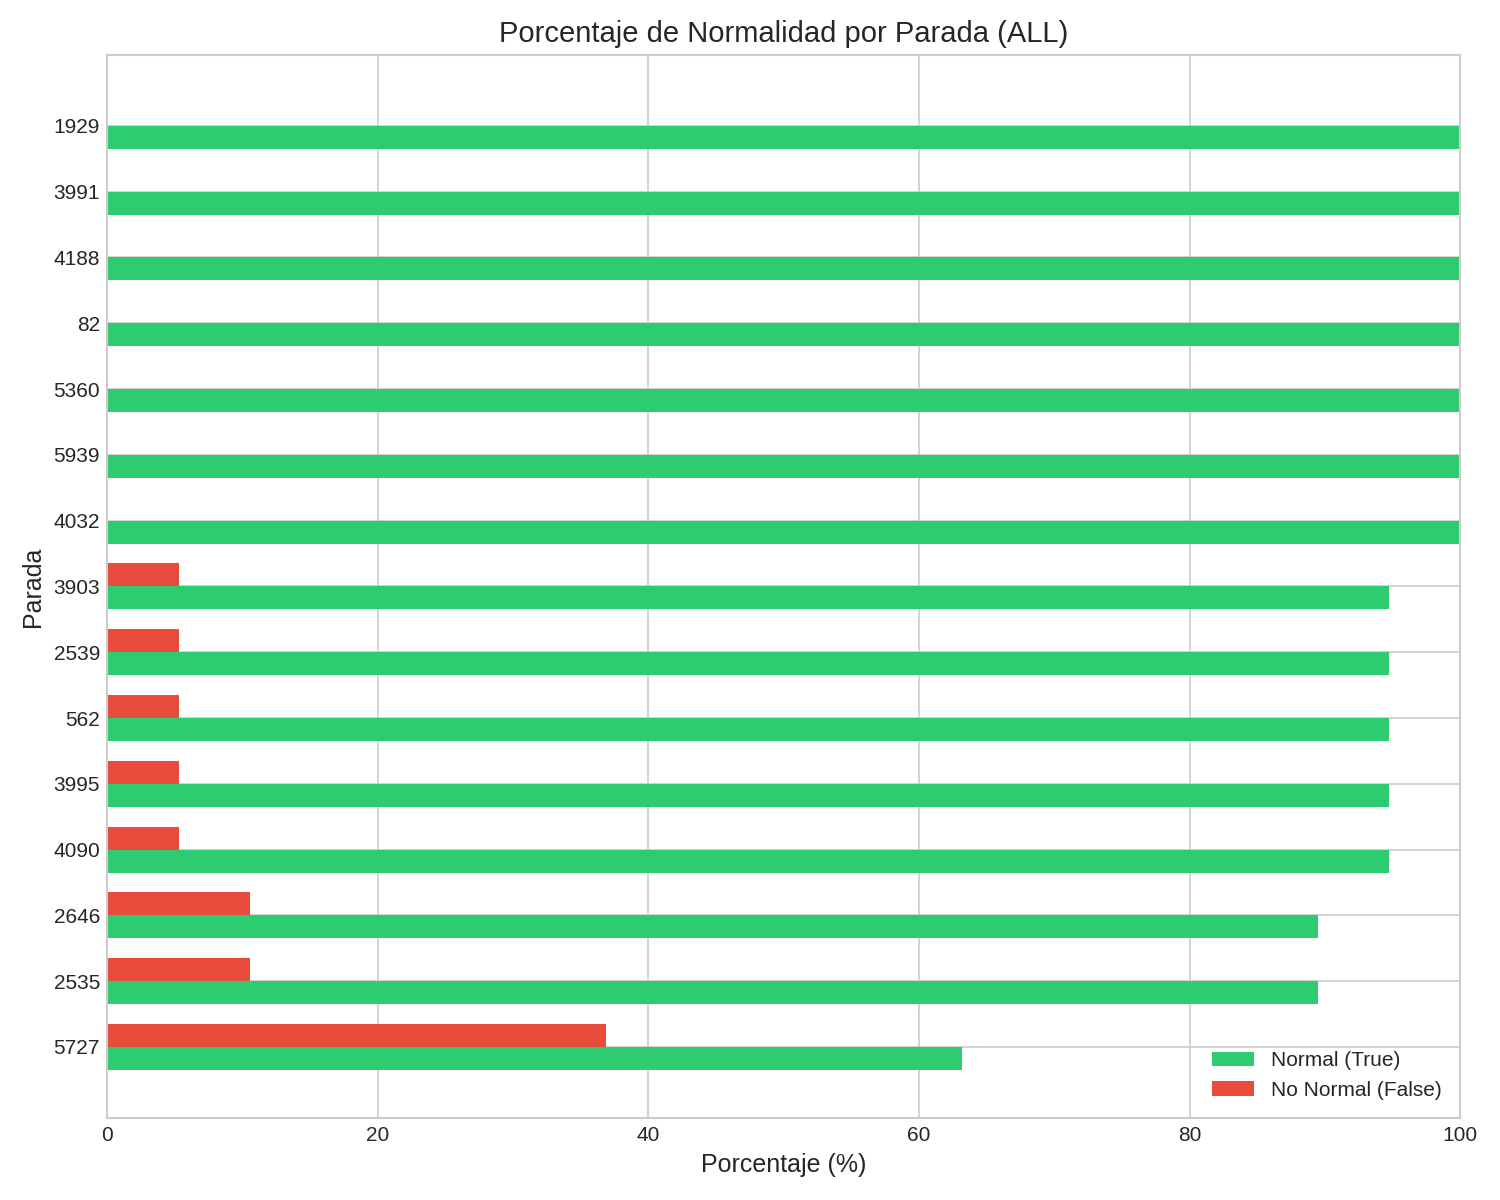
\includegraphics[width=\textwidth]{imagenes/to_A/normality_stop_ALL.png}
\caption{Porcentaje de no rechazo de hipótesis de normalidad por parada en sentido Cibeles con datos agregados.}
\par\vspace{4pt}{\footnotesize Fuente: elaboración propia.}\label{fig:normality_toA_all}
\end{figure}

\begin{figure}[H]
 \centering
    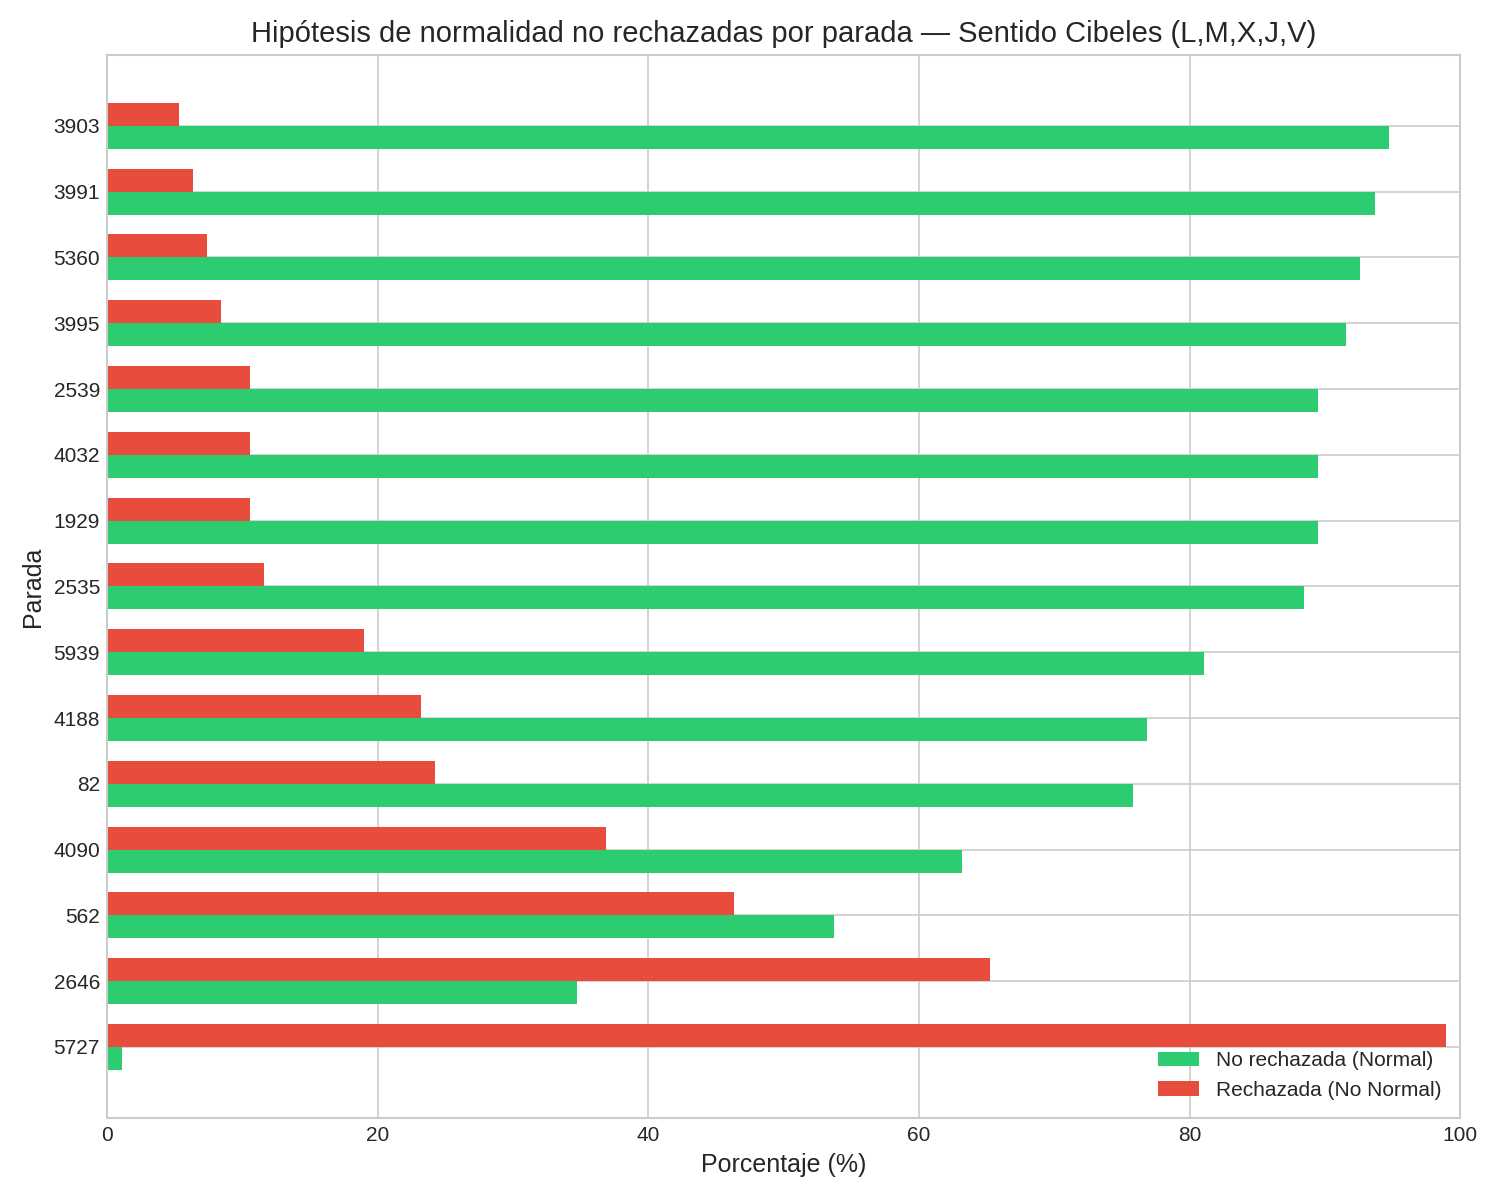
\includegraphics[width=\textwidth]{imagenes/to_A/normality_stop_individual.png}
\caption{Porcentaje de no rechazo de hipótesis de normalidad por parada en sentido Cibeles con datos desagregados.}
\par\vspace{4pt}{\footnotesize Fuente: elaboración propia.}\label{fig:normality_toA_deagregated}
\end{figure}

\begin{figure}[H]
 \centering
    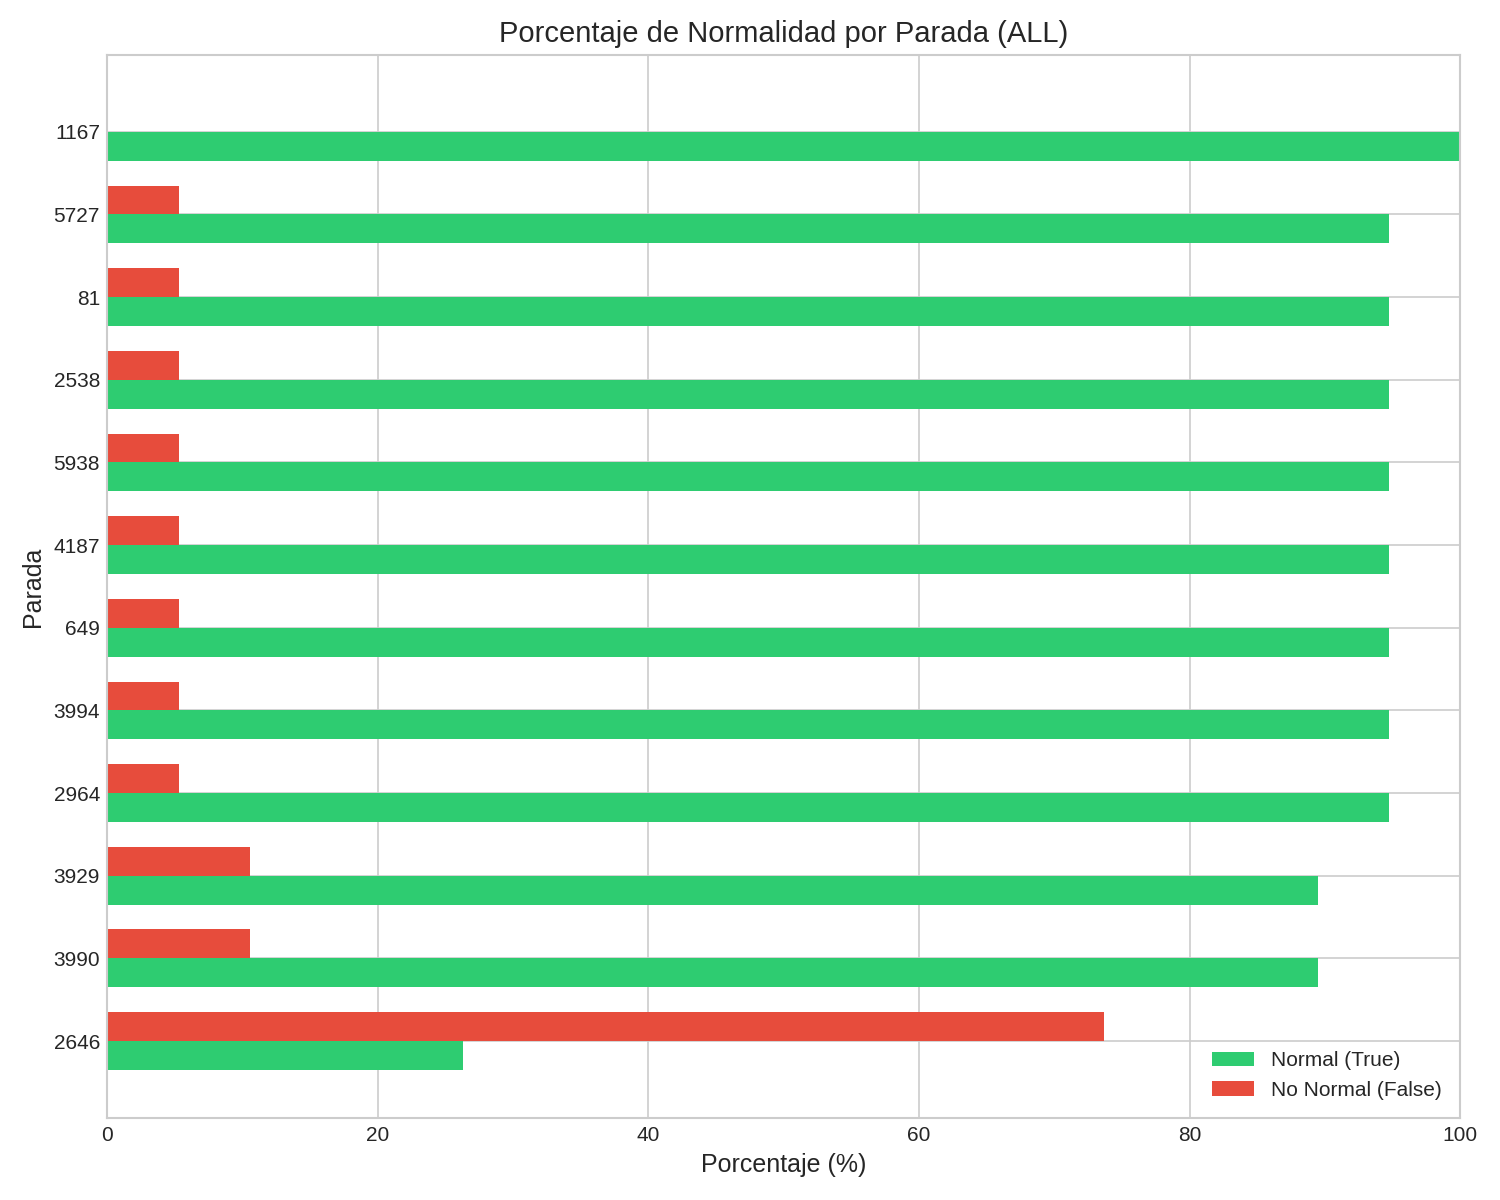
\includegraphics[width=\textwidth]{imagenes/to_B/normality_stop_ALL.png}
\caption{Porcentaje de no rechazo de hipótesis de normalidad por parada en sentido La Peseta con datos agregados.}
\par\vspace{4pt}{\footnotesize Fuente: elaboración propia.}\label{fig:normality_toB_all}
\end{figure}

\begin{figure}[H]
 \centering
    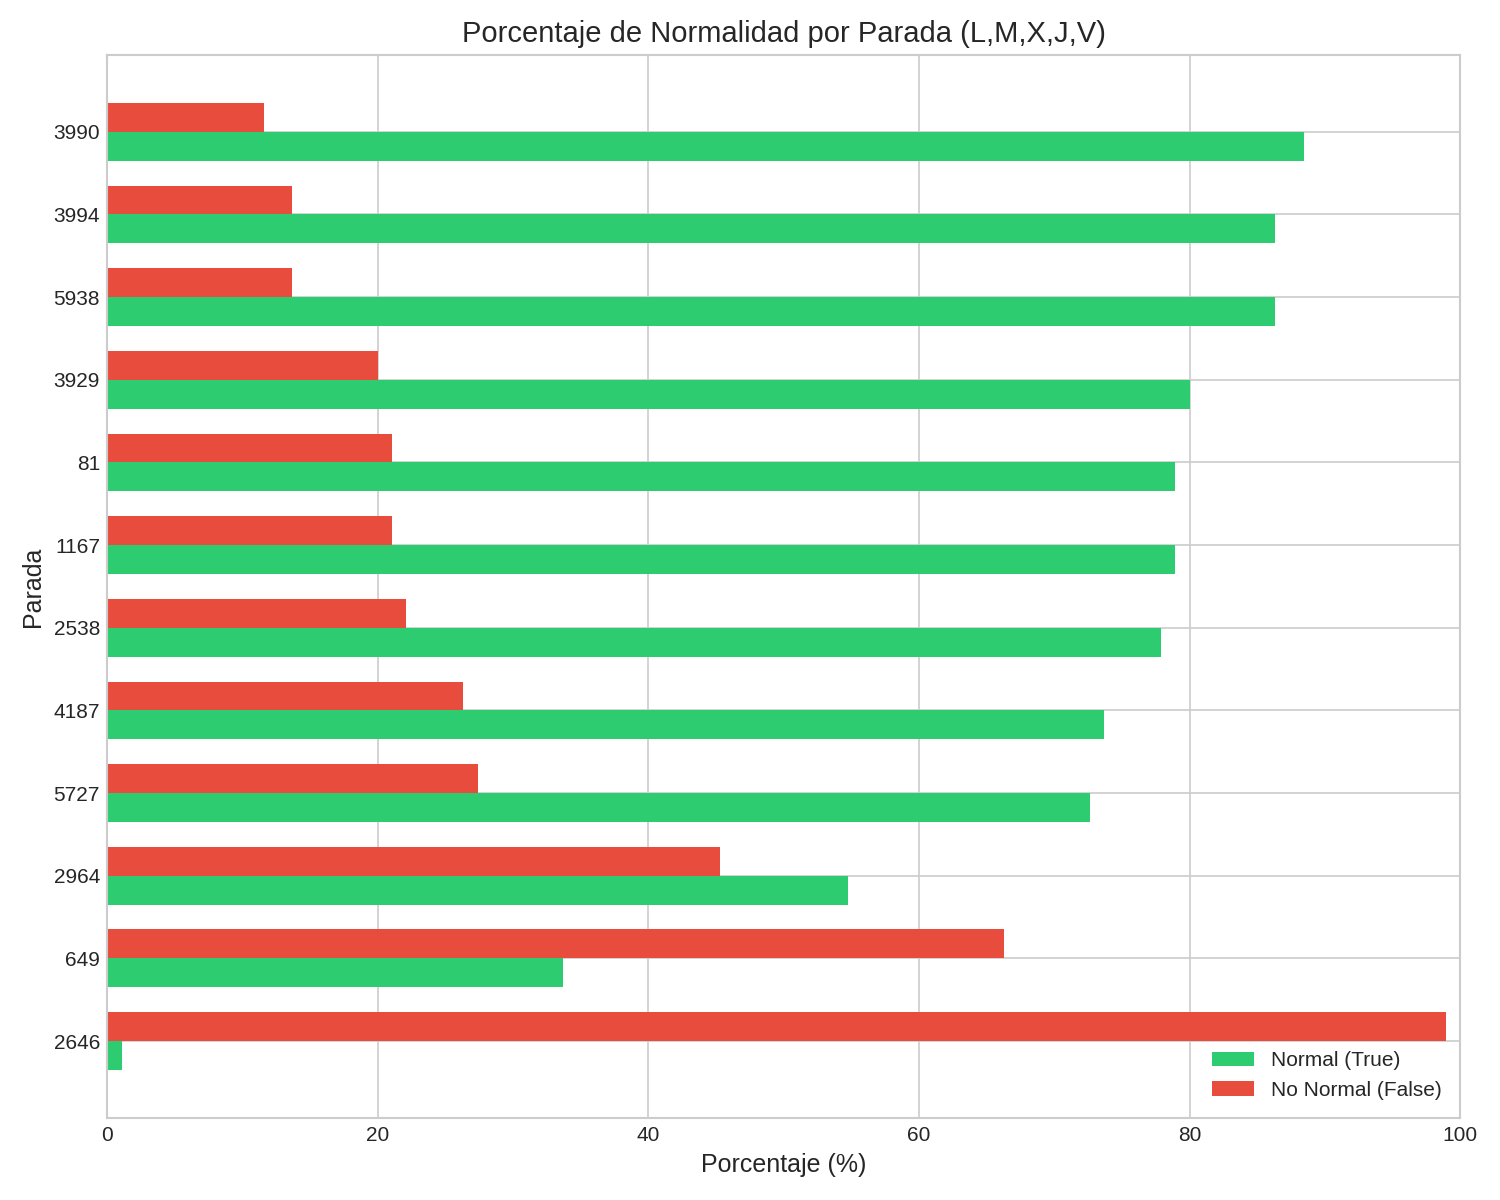
\includegraphics[width=\textwidth]{imagenes/to_B/normality_stop_individual.png}
\caption{Porcentaje de no rechazo de hipótesis de normalidad por parada en sentido La Peseta con datos desagregados.}
\par\vspace{4pt}{\footnotesize Fuente: elaboración propia.}\label{fig:normality_toB_deagregated}
\end{figure}

\chapter{Declaración de uso de IA generativa}\label{anex:iag}
% ---------------------------------------------------------------------------
% Anexo: Declaración de uso de Inteligencia Artificial Generativa (IAG)
% Transcripción a LaTeX del formulario oficial UC3M (TFG, curso 2026)
%
% Requiere en el preámbulo:
%   \usepackage{array}
%   \usepackage{tabularx}
%   \usepackage{amssymb}
%   \usepackage{enumitem}
%   \usepackage{hyperref}
% ---------------------------------------------------------------------------

% --- Macros auxiliares (colocar en el preámbulo, no aquí) ------------------
% Casilla vacía y casilla marcada
\newcommand{\casilla}{\makebox[1.4em][l]{$\square$}}
\newcommand{\casillam}{%
  \makebox[1.4em][l]{\rlap{$\square$}\hspace{0.17em}\raisebox{0.15ex}{\scriptsize$\checkmark$}}}
% Ancho útil de una celda que abarca las dos columnas de la tabla
\newcommand{\anchopleno}{\dimexpr\linewidth-2\tabcolsep-2\arrayrulewidth\relax}
% Estilo de las filas de enunciado
\newcolumntype{Y}{>{\raggedright\arraybackslash}X}


\begin{center}
  \textbf{\large DECLARACIÓN DE USO DE INTELIGENCIA ARTIFICIAL GENERATIVA (IAG)\\
  EN EL TRABAJO DE FIN DE GRADO (TFG)}
\end{center}

\bigskip

\noindent\textbf{He usado IAG en mi TFG}


\smallskip

\noindent\begin{tabularx}{\linewidth}{|Y|Y|}
\hline
\casillam\textbf{SÍ} & \casilla\textbf{NO} \\
\hline
\end{tabularx}


\section*{Parte 1: declaración sobre comportamiento legal, ético y responsable}

Ten presente que el uso de IAG conlleva unos riesgos y puede generar una serie de
consecuencias académicas graves: la evaluación de tu TFG puede verse comprometida si
el uso de la IAG comporta la utilización de datos de carácter confidencial, materiales
protegidos por derechos de autoría, o datos de carácter personal, y se hace sin cumplir
las condiciones exigidas en cada caso (autorización de los interesados, autorización de
los titulares, seguimiento de las instrucciones de la Universidad).

\medskip

\noindent\begin{tabularx}{\linewidth}{|Y|Y|}
\hline
\multicolumn{2}{|p{\anchopleno}|}{\textbf{Pregunta}} \\
\hline
\multicolumn{2}{|p{\anchopleno}|}{%
  \begin{minipage}[t]{\anchopleno}\vspace{2pt}
  \begin{enumerate}[label=\arabic*., leftmargin=1.6em, nosep, topsep=0pt]
    \item En mi interacción con herramientas de IAG he facilitado \textbf{datos de
      carácter confidencial} contando siempre con la debida autorización de los
      interesados. La confidencialidad abarca toda información que una persona u
      organización desea proteger por razones legales, comerciales, de privacidad o
      estratégicas (como patentes o secretos comerciales).
  \end{enumerate}
  \vspace{2pt}\end{minipage}} \\
\hline
\casilla SÍ, he usado estos datos con la autorización de los interesados
  & \casillam NO, no he usado datos de carácter confidencial \\
\hline
\multicolumn{2}{|p{\anchopleno}|}{%
  \begin{minipage}[t]{\anchopleno}\vspace{2pt}
  \begin{enumerate}[label=\arabic*., leftmargin=1.6em, nosep, topsep=0pt, start=2]
    \item En mi interacción con herramientas de IAG he facilitado \textbf{materiales
      protegidos por derechos de autoría} contando siempre con la autorización de los
      respectivos titulares.
  \end{enumerate}
  \vspace{2pt}\end{minipage}} \\
\hline
\casilla SÍ, he usado estos materiales con autorización de los titulares de derechos de
  autor; o bien sin ella porque se ajustan a una de las excepciones o límites que permite
  la ley:
  \begin{itemize}[leftmargin=1.2em, nosep, topsep=2pt]
    \item obra en dominio público
    \item obra licenciada (licencias Creative Commons)
    \item uso de fragmentos con fines de investigación (derecho de cita)
  \end{itemize}
  & \casillam NO, no he usado materiales protegidos por derechos de autoría \\
\hline
\multicolumn{2}{|p{\anchopleno}|}{%
  \begin{minipage}[t]{\anchopleno}\vspace{2pt}
  \begin{enumerate}[label=\arabic*., leftmargin=1.6em, nosep, topsep=0pt, start=3]
    \item En mi interacción con herramientas de IAG he facilitado \textbf{datos de
      carácter personal} con la debida autorización de los interesados.
  \end{enumerate}
  \vspace{2pt}\end{minipage}} \\
\hline
\casilla SÍ, he usado estos datos con autorización de los interesados y conforme a las
  instrucciones contenidas en la
  \href{https://docs.google.com/document/d/1YghVxFwo8a1VqdfnvJiZzlmAkfYepbDmD4g3hTOW9ro/edit?tab=t.0}{guía aprobada por la Universidad}
  & \casillam NO, no he usado datos de carácter personal \\
\hline
\multicolumn{2}{|p{\anchopleno}|}{%
  \begin{minipage}[t]{\anchopleno}\vspace{2pt}
  \begin{enumerate}[label=\arabic*., leftmargin=1.6em, nosep, topsep=0pt, start=4]
    \item Mi utilización de la herramienta de IAG ha \textbf{respetado sus términos de
      uso}, así como los principios éticos esenciales, no orientándola de manera
      maliciosa a obtener un resultado inapropiado para el trabajo presentado, es decir,
      que produzca una impresión o conocimiento contrario a la realidad de los resultados
      obtenidos, que suplante mi propio trabajo o que pueda resultar en un perjuicio para
      las personas.
  \end{enumerate}
  \vspace{2pt}\end{minipage}} \\
\hline
\casillam SÍ & \casilla NO \\
\hline
\end{tabularx}

\section*{Parte 2: declaración de uso técnico}

Utiliza el siguiente modelo de declaración tantas veces como sea necesario, a fin de
reflejar todos los tipos de iteración que has tenido con herramientas de IAG. Incluye un
ejemplo por cada tipo de uso realizado.

\medskip

\noindent\textbf{Declaro haber hecho uso del sistema de IAG} (Claude, de Anthropic, modelos de la
familia Claude, versiones disponibles entre 2025 y 2026) \textbf{para:}

\subsection*{Documentación y redacción}

\begin{itemize}[leftmargin=1.4em]
  \item Soporte a la reflexión en relación con el desarrollo del trabajo: proceso
    iterativo de análisis de alternativas y enfoques utilizando la IAG.

  Se ha empleado la herramienta para someter el documento a una revisión crítica sistemática frente a la matriz de evaluación, \textbf{empleando el prompt} 
  \enquote{actúa como catedrático y miembro de un tribunal evaluador exigente; audita el documento adjunto frente a la matriz de evaluación}, 
  \textbf{teniendo como interacción} un proceso iterativo de contraste en el que se aceptaron parte de las observaciones y se rebatieron y descartaron otras.

  \item Revisión o reescritura de párrafos redactados previamente.

  Se ha empleado la herramienta para la revisión de redacción de fragmentos ya escritos con el fin de encontrar inconsistencias en el texto redactado y posibles faltas ortográficas.

  \item Búsqueda de información o respuesta a preguntas concretas.
  
  Se ha empleado la herramienta para realizar consultas puntuales sobre convenciones de citación, formalización de contrastes estadísticos y errores de compilación en \LaTeX.
\end{itemize}

\subsection*{Desarrollar contenido específico}

Se ha hecho uso de IAG como herramienta de soporte para el desarrollo del contenido
específico del TFG, incluyendo:

\begin{itemize}[leftmargin=1.4em]
  \item Asistencia en el desarrollo de líneas de código (programación).
  
  Depuración de errores en el código \LaTeX y revisión de fragmentos de código Python del análisis de datos.

  \item Tratamiento de datos: recogida, análisis, cruce de datos.

  Verificación de cálculos y contraste de decisiones metodológicas sobre el ajuste de distribuciones.
\end{itemize}



\section*{Parte 3: reflexión sobre utilidad}

% Valoración personal (formato libre) sobre fortalezas y debilidades identificadas en el
% uso de herramientas de IAG durante el desarrollo del trabajo: utilidad en el proceso de
% aprendizaje, en el desarrollo y en la extracción de conclusiones.

El uso de estas herramientas ha resultado especialmente útil en la fase de revisión crítica del documento,
al permitir un contraste sistemático frente a los criterios de evaluación que difícilmente se obtiene mediante
relectura propia. Su utilidad ha sido, en cambio, limitada en las decisiones metodológicas de fondo, ya que varias de las
observaciones recibidas partían de premisas incorrectas sobre el trabajo y era necesario rebatirlas y descartarlas, lo que
exigió mantener en todo momento el criterio propio como instancia última de decisión. La conclusión que se extrae es que
estas herramientas resultan valiosas como interlocutor crítico y como apoyo en tareas instrumentales, pero no sustituyen el
juicio técnico del autor sobre el dominio del problema.
\end{document}